\tableofcontents

\pagebreak

\section{Построение математической модели объекта}
\subsection{Вывод уравнений}
\begin{figure}[]
    \centering
    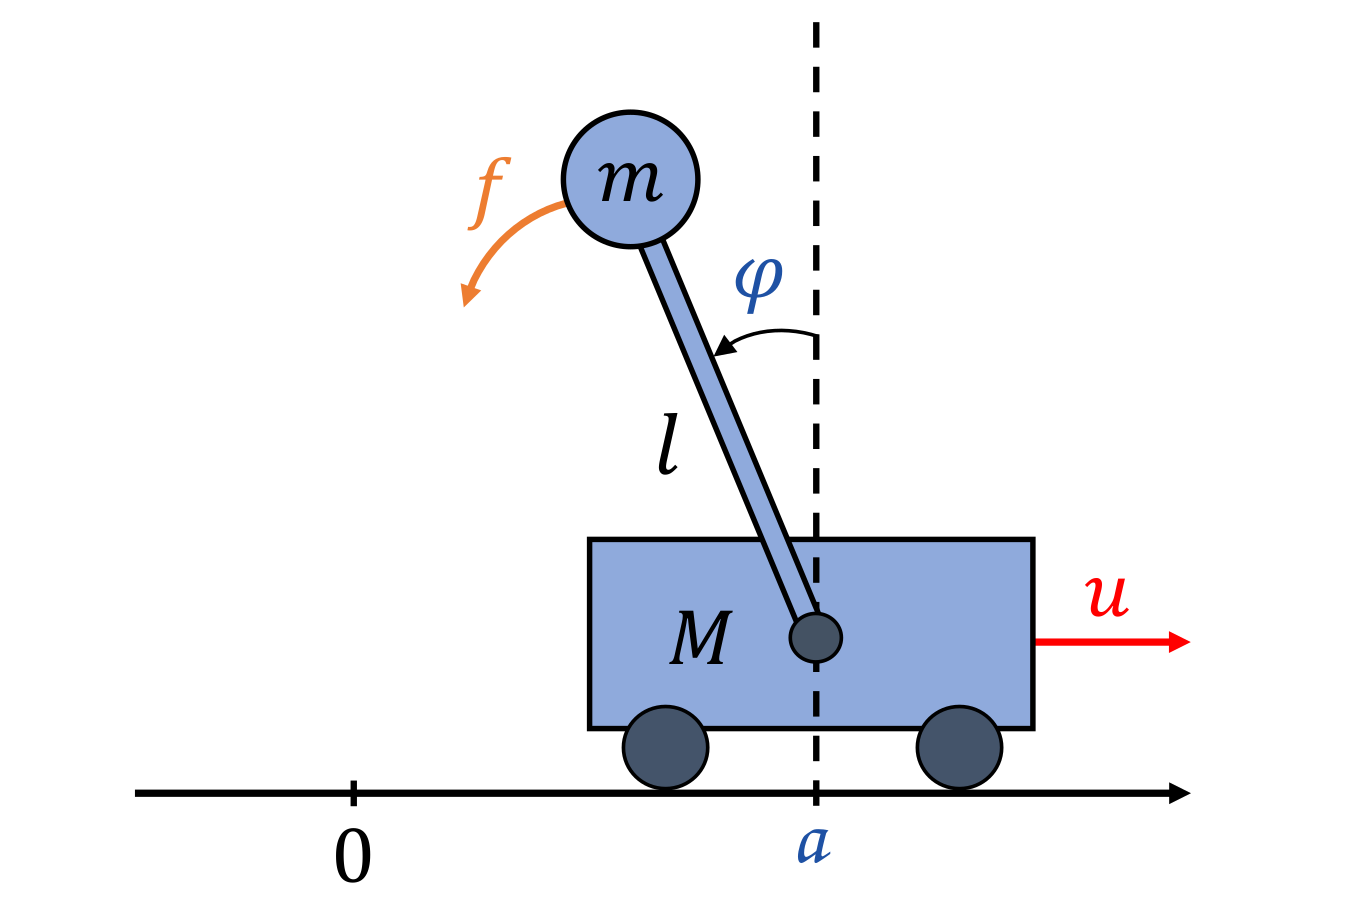
\includegraphics[width=300px]{pendulum.png}
    \caption{\label{fig:task1_1}Перевернутый маятник на тележке.}
\end{figure}

Рассмотрим систему перевернутого маятника на тележке (рис. \ref{fig:task1_1}). Введем следущие обозначения физических величин:
\begin{itemize}
    \item $a$ -- линейная координата тележки;
    \item $\dot{a}$ -- линейная скорость тележки;
    \item $\varphi$ -- угол отклонения маятника от вертикали;
    \item $\dot{\varphi}$ -- угловая скорость маятника;
    \item $f$ -- вращающий внешний момент, действующий на маятник;
    \item $u$ -- сила действующая на тележку;
    \item $M, m$ --  массы тележки и маятника соответственно;
    \item $l$ -- длина маятника.
\end{itemize}

В качестве вектора состояния $x = \begin{bmatrix}
    x_1 & x_2 & x_3 & x_4
\end{bmatrix}^T$ выберем набор $a, \dot{a}, \varphi, \dot{\varphi}$. В роли управляющего воздействия примем $u$, в роли внешнего возмущения -- $f$.
Измеряемыми сигналами $y = \begin{bmatrix}
    y_1 & y_2
\end{bmatrix}^T$ будем считать $a$ и $\varphi$.
\begin{equation} \label{eq:1}
    \begin{cases}
        x_1 = a \\ x_2 = \dot{a} \\ x_3 = \varphi \\ x_4 = \dot{\varphi} \\ y_1 = a \\ y_2 = \varphi
    \end{cases}
\end{equation}

Для вывода математической модели данной физической системы воспользуемся уравнениями Лагранжа:
\begin{equation} \label{eq:2}
    \begin{cases}
        \frac{d}{dt}\frac{\partial T}{\partial \dot{a}} - \frac{\partial T}{\partial a} = u \\
        \frac{d}{dt}\frac{\partial T}{\partial \dot{\varphi}} - \frac{\partial T}{\partial \varphi} = f + mgl\sin(\varphi)
    \end{cases},
\end{equation}
где $T$ -- кинетическая энергия системы.
\begin{equation} \label{eq:3}
    T(t) = M\frac{\dot{a}^2}{2} + m\frac{(\frac{d}{dt}(l\cos(\varphi)))^2 + (-\frac{d}{dt}(l\sin(\varphi)) + \dot{a})^2}{2}=
    (M+m)\frac{\dot{a}^2}{2} + \frac{ml^2\dot{\varphi}^2}{2} - ml\cos(\varphi)\dot{a}\dot{\varphi}
\end{equation}
Подставив выражение для $T$ в уравнения \ref{eq:2}, получим уравнения математической модели системы:
\begin{equation} \label{eq:4}
    \begin{cases}
        (M+m)\ddot{a} + ml(\sin(\varphi)\dot{\varphi}^2 - \cos(\varphi)\ddot{\varphi}) = u \\
        ml^2\ddot{\varphi} - ml\ddot{a}\cos{\varphi} = f + mgl\sin(\varphi)
    \end{cases}
\end{equation}
Тогда, выразив $\ddot{a}$ и $\ddot{\varphi}$:
\begin{equation} \label{eq:5}
    \begin{cases}
        \ddot a = -\frac{ml}{M+m}\sin(\varphi)\dot{\varphi}^2 + \frac{ml}{M+m}\cos(\varphi)\ddot{\varphi} + \frac{1}{M+m}u \\
        \ddot \varphi = \frac{1}{l}\ddot a \cos(\varphi) + \frac{g}{l}\sin(\varphi) + \frac{1}{ml^2}f
    \end{cases}
\end{equation}
Решив данную систему уравнений \ref{eq:5} относительно $\ddot a$ и $\ddot \varphi$:
\begin{equation} \label{eq:6}
    \begin{cases}
        \ddot a = \frac{1}{M + m\sin(\varphi)^2}( -ml\sin(\varphi)\dot{\varphi}^2 + mg\cos(\varphi)\sin(\varphi) + \frac{\cos(\varphi)}{l}f + u ) \\
        \ddot \varphi = \frac{1}{M + m\sin(\varphi)^2}( -m\sin(\varphi)\cos(\varphi)\dot{\varphi}^2 + \frac{(M+m)g}{l}\sin(\varphi) + \frac{M+m}{ml^2}f + \frac{\cos(\varphi)}{l}u )
    \end{cases}
\end{equation}

Представим математическую модель в терминах вектора состояния:
\begin{equation} \label{eq:7}
    \begin{cases}
        \dot x_1 = x_2 \\
        \dot x_2 = \frac{1}{M + m\sin(x_3)^2}( -ml\sin(x_3)x_4^2 + mg\cos(x_3)\sin(x_3) + \frac{\cos(x_3)}{l}f + u ) \\
        \dot x_3 = x_4 \\
        \dot x_4 = \frac{1}{M + m\sin(x_3)^2}( -m\sin(x_3)\cos(x_3)x_4^2 + \frac{(M+m)g}{l}\sin(x_3) + \frac{M+m}{ml^2}f + \frac{\cos(x_3)}{l}u ) \\
        y_1 = x_1 \\
        y_2 = x_3
    \end{cases}
\end{equation}

\subsection{Точки равновесия}
В точках равновесия все компоненты производной вектора состояния по времени равны $0$. Следовательно, полагая $u, f \equiv 0$
необходимо:
\begin{equation} \label{eq:8}
    \begin{cases}
        x_2 = 0 \\
        \frac{1}{M + m\sin(x_3)^2}( -ml\sin(x_3)x_4^2 + mg\cos(x_3)\sin(x_3) ) = 0 \\
        x_4 = 0 \\
        \frac{1}{M + m\sin(x_3)^2}( -m\sin(x_3)\cos(x_3)x_4^2 + \frac{(M+m)g}{l}\sin(x_3) ) = 0 \\
    \end{cases}
\end{equation}
Учитывая $x_4 = 0$ и $M + m\sin(x_3)^2 > 0$:
\begin{equation} \label{eq:9}
    \begin{cases}
        x_1 \in \mathbb{R} \\
        x_2 = 0 \\
        x_3 = \pi n, n \in \mathbb{Z} \\ 
        x_4 = 0 
    \end{cases}
\end{equation}
Заметим, однако, что с физической точки зрения условие $x_3 = \pi n$ эквивалентно $x_3 = 0$ (верхнее положение маятника) или $x_3 = \pi$ (нижнее положение маятника). В дальнейшем нас будет интересовать стабилизация системы около верхенего положения равновесия.

\subsection{Линеаризация}
Для линеаризации системы около векхней точки равновесия ($x = \begin{bmatrix}
    a_0 & 0 & 0 & 0
\end{bmatrix}^T$) представим некоторые функции от компонент вектора состояния в виде ряда Тейлора в данной точке:
\begin{equation*}\sin(x_3) = x_3 + \sum_{n=1}^{\infty}(-1)^n\frac{x_3^{2n+1}}{(2n+1)!}\end{equation*}
\begin{equation*}\cos(x_3) = 1 + \sum_{n=1}^{\infty}(-1)^n\frac{x_3^{2n}}{(2n)!}\end{equation*}
Приняв величины вектора состояния достаточно малыми ($x_3^2 \ll x_3$, $x_4^2 \ll x_4$), можем записать линеаризованные уравненя динамики системы:
\begin{equation} \label{eq:10}
    \begin{cases}
        \dot x_1 = x_2 \\
        \dot x_2 = \frac{mg}{M}x_3 + \frac{1}{Ml}f + \frac{1}{M}u \\
        \dot x_3 = x_4 \\
        \dot x_4 = \frac{(m+m)g}{Ml}x_3 + \frac{M+m}{Mml^2}f + \frac{1}{Ml}u \\
    \end{cases}
\end{equation}

Можем представить линеаризованную систему в матричном виде:
\begin{equation} \label{eq:11}
    \begin{cases}
        \dot x = Ax + Bu + Df \\
        y = Cx
    \end{cases},
\end{equation}
где матрицы $A$, $B$, $C$, $D$ имеют следующий вид:
\begin{equation*}
    A = \begin{bmatrix}
        0 & 1 & 0 & 0 \\
        0 & 0 & \frac{mg}{M} & 0 \\
        0 & 0 & 0 & 1 \\
        0 & 0 & \frac{(M+m)g}{Ml} & 0
    \end{bmatrix},
    B = \begin{bmatrix}
        0 \\ \frac{1}{M} \\ 0 \\ \frac{1}{Ml}
    \end{bmatrix},
    D = \begin{bmatrix}
        0 \\ \frac{1}{Ml} \\ 0 \\ \frac{M+m}{Mml^2}
    \end{bmatrix},
    C = \begin{bmatrix}
        1 & 0 & 0 & 0 \\
        0 & 0 & 1 & 0
    \end{bmatrix}
\end{equation*}

Выберем значения параметров системы:
\begin{equation*}
    M = 10, m = 1, l = 1, g = 9.8
\end{equation*}
Тогда, матрицы системы примут следующий вид:
\begin{equation*}
    A = \begin{bmatrix}
        0 & 1 & 0 & 0 \\
        0 & 0 & 0.98 & 0 \\
        0 & 0 & 0 & 1 \\
        0 & 0 & 10.78 & 0
    \end{bmatrix},
    B = \begin{bmatrix}
        0 \\ 0.1 \\ 0 \\ 0.1
    \end{bmatrix},
    D = \begin{bmatrix}
        0 \\ 0.1 \\ 0 \\ 1.1
    \end{bmatrix},
    C = \begin{bmatrix}
        1 & 0 & 0 & 0 \\
        0 & 0 & 1 & 0
    \end{bmatrix}
\end{equation*}
\pagebreak

\section{Анализ математической модели}
\subsection{Анализ матриц}
Найдем собственные числа и собственные вектора матрицы $A$:
\begin{equation*}
    \sigma(A) = \{0, 0, 3.28, -3.28\}; \nu(A) = \{\begin{bmatrix}
        1 \\ 0 \\ 0 \\ 0
    \end{bmatrix},
    \begin{bmatrix}
        -1 \\ 0 \\ 0 \\ 0
    \end{bmatrix},
    \begin{bmatrix}
        0.026 \\ 0.087 \\ 0.29 \\ 0.953
    \end{bmatrix},
    \begin{bmatrix}
        -0.026 \\ 0.087 \\ -0.29 \\ 0.953
    \end{bmatrix}\}
\end{equation*}
Заметим, что первые два собственных вектора линейно зависимы и соответствуют нулевым собственным числам. Можем сделать вывод,
что первая компонента вектора состояния не влияет на динамику системы (от координаты тележки не зависят другие параметры и их производные).

Имея кратные нулевые корни, а также положительное собственное число, система является неустойчивой. Проведем анализ на управляемость, стабилизируемость, наблюдаемость и обнаруживаемость приведя систему в Жорданов базис:
\begin{equation*}
    A = PJP^{-1} = \begin{bmatrix}
        1 & 0 & -0.03 & 0.03 \\
        0 & 1 & 0.09 & 0.09 \\
        0 & 0 & -0.31 & 0.31 \\
        0 & 0 & 1 & 1
    \end{bmatrix}
    \begin{bmatrix}
        0 & 1 & 0 & 0 \\
        0 & 0 & 0 & 0 \\
        0 & 0 & -3.28 & 0 \\
        0 & 0 & 0 & 3.28
    \end{bmatrix}
    \begin{bmatrix}
        1 & 0 & -0.03 & 0.03 \\
        0 & 1 & 0.09 & 0.09 \\
        0 & 0 & -0.31 & 0.31 \\
        0 & 0 & 1 & 1
    \end{bmatrix}^{-1}
\end{equation*}
\begin{equation*}
    P^{-1}B = \begin{bmatrix}
        0 \\ 0.09 \\ 0.05 \\ 0.05
    \end{bmatrix},
    CP = \begin{bmatrix}
        1 & 0 & -0.03 & 0.03 \\
        0 & 0 & -0.31 & 0.31
    \end{bmatrix}
\end{equation*}
Можем сделать вывод, что система является полностью управляемой и наблюдаемой (соответственно стабилизируемой и обнаруживаемой).

\subsection{Передаточные функции}
Найдем передаточные матрицы системы от входа к выходу и от внешнего возмущения к выходу:
\begin{equation*}
    \underset{u\to y}{W}(s) = \begin{bmatrix}
        \frac{0.1s^2 - 0.98}{s^4 - 10.78s^2} \\
        \frac{0.1}{s^2 - 10.78}
    \end{bmatrix}, 
    \underset{f\to y}{W}(s) = \begin{bmatrix}
        \frac{0.1}{s^2 - 10.78} \\
        \frac{1.1}{s^2 - 10.78}
    \end{bmatrix}
\end{equation*}
Динамический порядок функции $\frac{0.1s^2 - 0.98}{s^4 - 10.78s^2}$ равен $4$, для остальных -- $2$. Относительный динамический порядок всех функций равен $2$.
Нули присутствуют только у функции $\frac{0.1s^2 - 0.98}{s^4 - 10.78s^2}$ и равны $\pm 3.13$. Полюса передаточных функций соответствуют собственным числам матрицы динамики системы.

Все функции описывают расходящийся переходный процесс при нулевом входном (внешнем) воздействии, т.к. имеют кратные нулевые или положительный полюса.

\subsection{Линейное моделирование}
Выполним моделирование линеаризованной системы, заданной уравнениями \ref{eq:11}.
Ниже приведены графики, демонстрирующие динамику вектора состояния при различных начальных условиях.

\begin{figure}[]
    \centering
    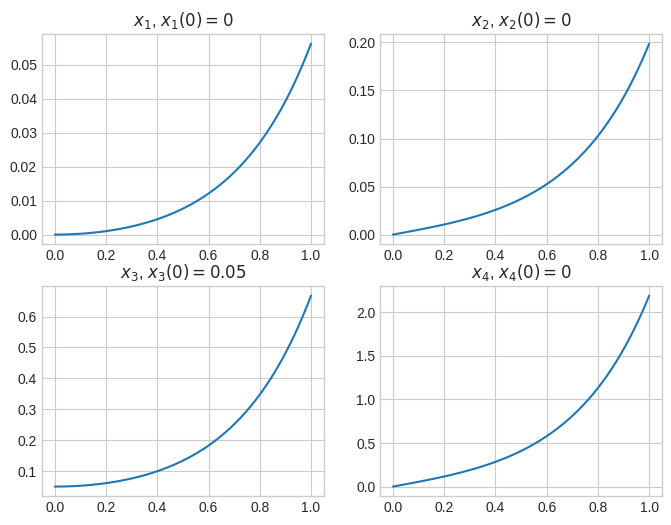
\includegraphics[width=300px]{state_lin_1.png}
    \caption{\label{fig:task2_3_1}Моделирование линеаризованной системы ($x(0)=\begin{bmatrix}
        0 & 0 & 0.05 & 0
    \end{bmatrix}^T$).}
\end{figure}

\begin{figure}[]
    \centering
    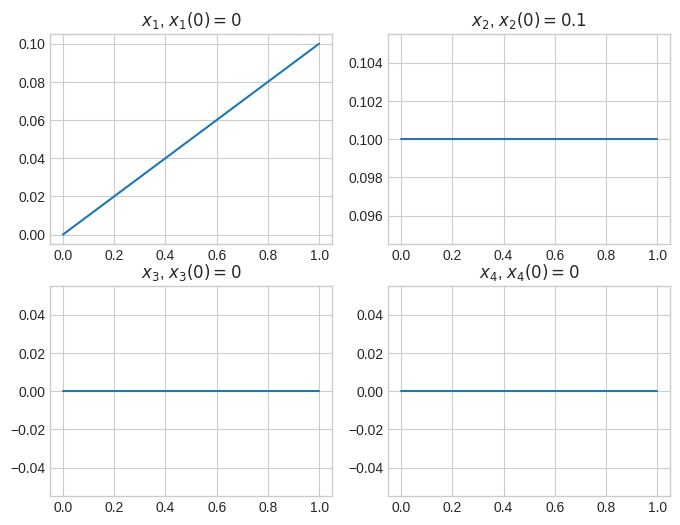
\includegraphics[width=300px]{state_lin_2.png}
    \caption{\label{fig:task2_3_2}Моделирование линеаризованной системы ($x(0)=\begin{bmatrix}
        0 & 0.1 & 0 & 0
    \end{bmatrix}^T$).}
\end{figure}

\begin{figure}[]
    \centering
    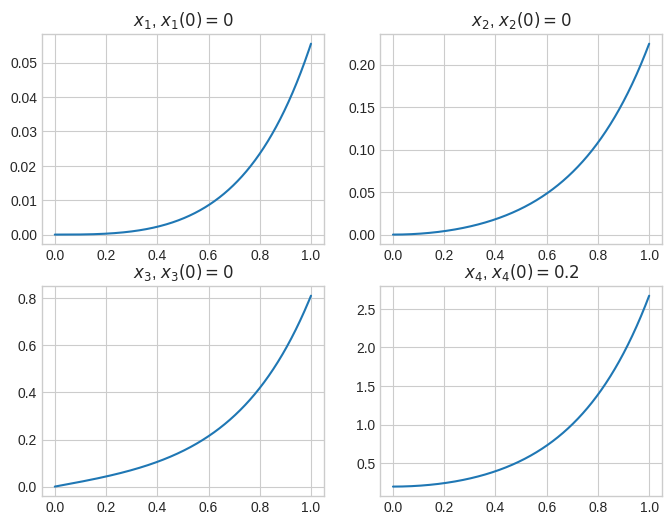
\includegraphics[width=300px]{state_lin_3.png}
    \caption{\label{fig:task2_3_3}Моделирование линеаризованной системы ($x(0)=\begin{bmatrix}
        0 & 0 & 0 & 0.2
    \end{bmatrix}^T$).}
\end{figure}

\begin{figure}[]
    \centering
    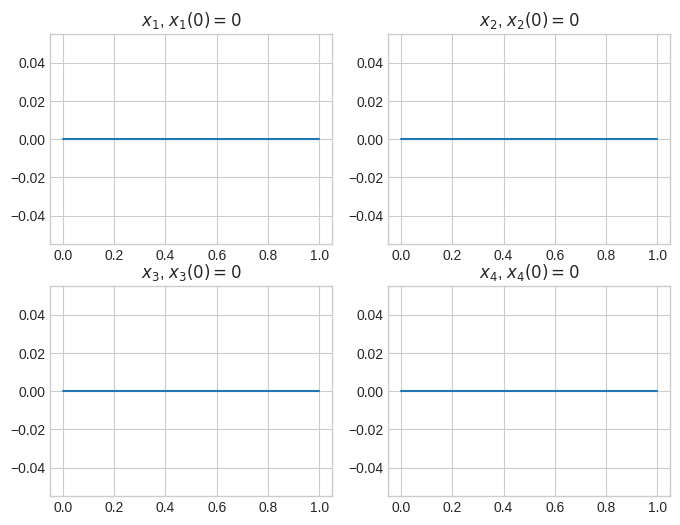
\includegraphics[width=300px]{state_lin_4.png}
    \caption{\label{fig:task2_3_4}Моделирование линеаризованной системы ($x(0)=\begin{bmatrix}
        0 & 0 & 0 & 0
    \end{bmatrix}^T$).}
\end{figure}

\subsection{Нелинейное моделирование}
Выполним моделирование исходной системы, заданной уравнениями \ref{eq:7}.
Ниже приведены графики, демонстрирующие динамику вектора состояния при различных начальных условиях.

\begin{figure}[]
    \centering
    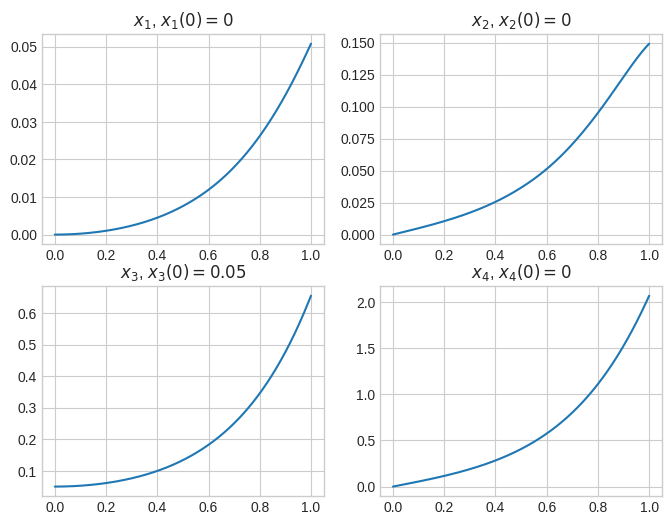
\includegraphics[width=300px]{state_nonlin_1.png}
    \caption{\label{fig:task2_4_1}Моделирование исходной системы ($x(0)=\begin{bmatrix}
        0 & 0 & 0.05 & 0
    \end{bmatrix}^T$).}
\end{figure}

\begin{figure}[]
    \centering
    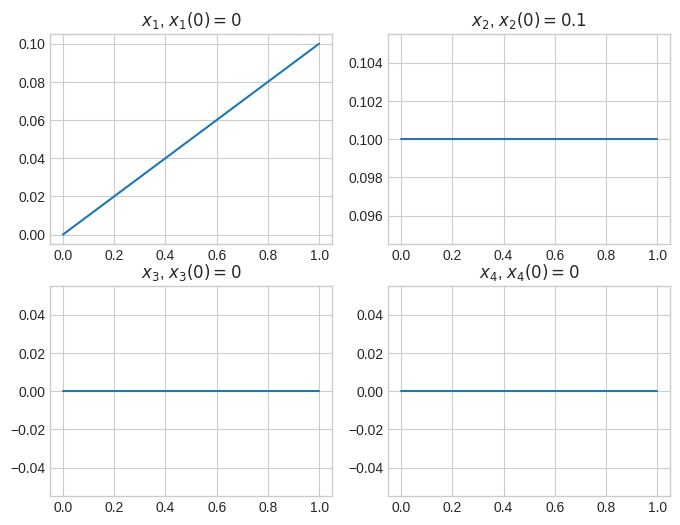
\includegraphics[width=300px]{state_nonlin_2.png}
    \caption{\label{fig:task2_4_2}Моделирование исходной системы ($x(0)=\begin{bmatrix}
        0 & 0.1 & 0 & 0
    \end{bmatrix}^T$).}
\end{figure}

\begin{figure}[]
    \centering
    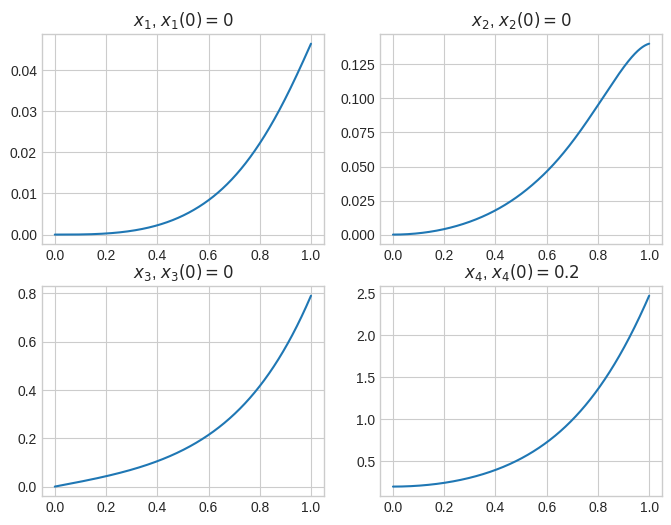
\includegraphics[width=300px]{state_nonlin_3.png}
    \caption{\label{fig:task2_4_3}Моделирование исходной системы ($x(0)=\begin{bmatrix}
        0 & 0 & 0 & 0.2
    \end{bmatrix}^T$).}
\end{figure}

\begin{figure}[]
    \centering
    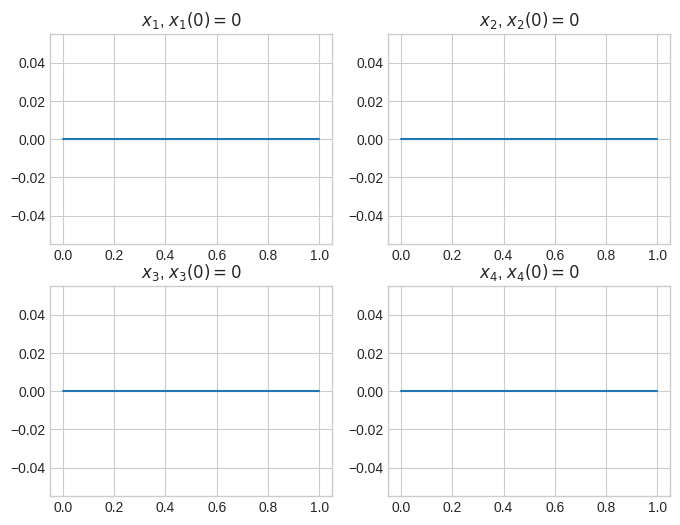
\includegraphics[width=300px]{state_nonlin_4.png}
    \caption{\label{fig:task2_4_4}Моделирование исходной системы ($x(0)=\begin{bmatrix}
        0 & 0 & 0 & 0
    \end{bmatrix}^T$).}
\end{figure}
\pagebreak
Заметим, что при малом времени моделирования динамика систем очень схожая. Построим сравнительные графики при большем времени переходного процесса.

\begin{figure}[]
    \centering
    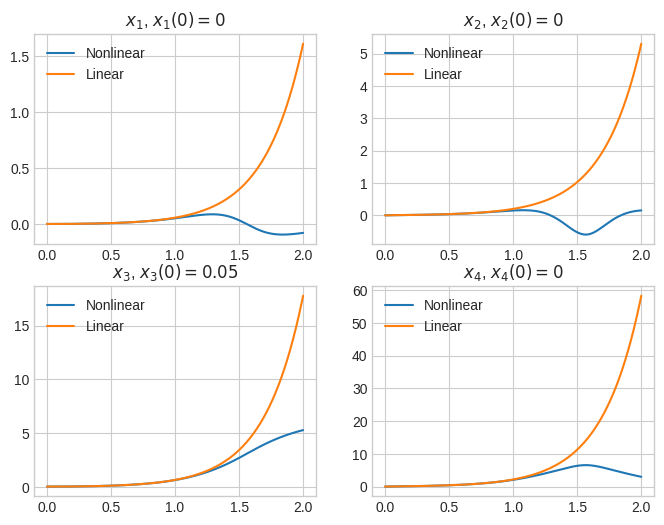
\includegraphics[width=300px]{state_lin_nonlin_1.png}
    \caption{\label{fig:task2_4_5}Сравнительное моделирование систем ($x(0)=\begin{bmatrix}
        0 & 0 & 0.05 & 0
    \end{bmatrix}^T$).}
\end{figure}

\begin{figure}[]
    \centering
    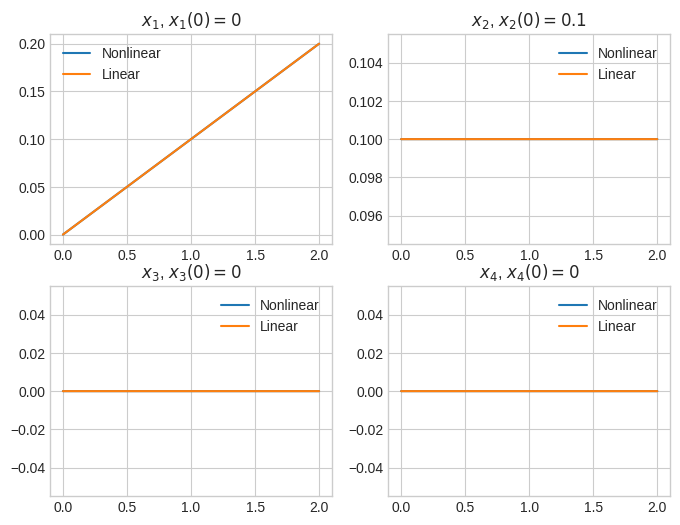
\includegraphics[width=300px]{state_lin_nonlin_2.png}
    \caption{\label{fig:task2_4_6}Сравнительное моделирование систем ($x(0)=\begin{bmatrix}
        0 & 0.1 & 0 & 0
    \end{bmatrix}^T$).}
\end{figure}

\begin{figure}[]
    \centering
    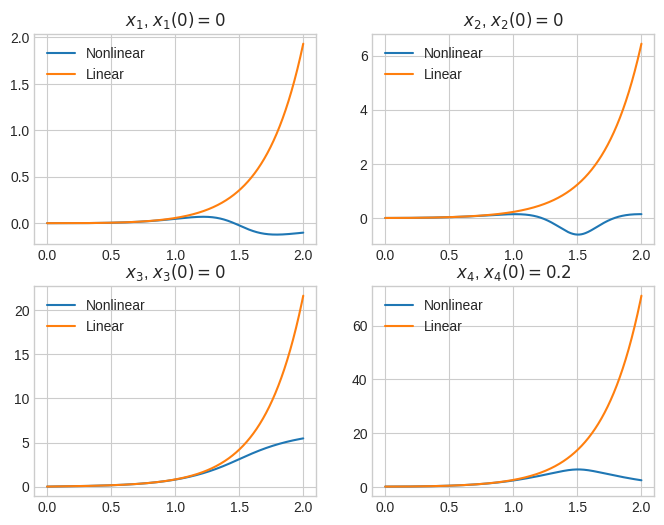
\includegraphics[width=300px]{state_lin_nonlin_3.png}
    \caption{\label{fig:task2_4_7}Сравнительное моделирование систем ($x(0)=\begin{bmatrix}
        0 & 0 & 0 & 0.2
    \end{bmatrix}^T$).}
\end{figure}

\begin{figure}[]
    \centering
    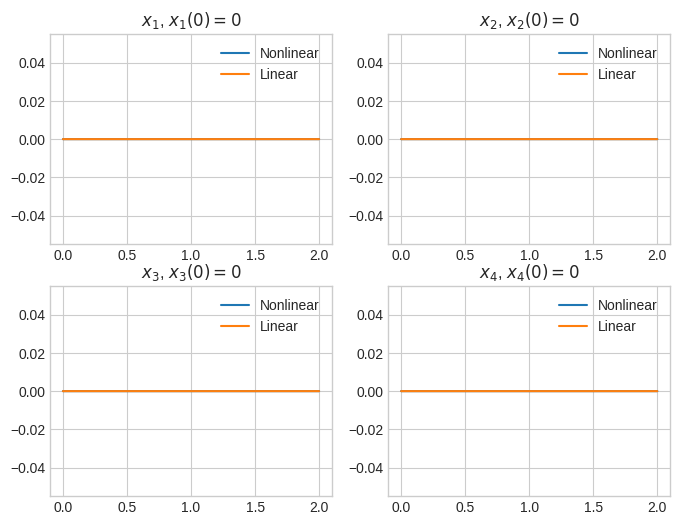
\includegraphics[width=300px]{state_lin_nonlin_4.png}
    \caption{\label{fig:task2_4_8}Сравнительное моделирование систем ($x(0)=\begin{bmatrix}
        0 & 0 & 0 & 0
    \end{bmatrix}^T$).}
\end{figure}

\pagebreak
При увеличении времени моделирования расхождения становятся явно заметными.

\section{Модальное управление}

\subsection{Синтез регулятора по состоянию}
В этом задании выводится модальный регулятор для системы:
\begin{equation}
    \begin{cases}
        \dot{x} = A x + Bu \\
        u = K x \\
\end{cases} 
\end{equation}

Выберем матрицу $\Gamma \in \mathbb{R}^{n \times n}$ с желаемым спектром. Найдем $K$ такое, что $A+BK = P \Gamma P^{-1}$.
Для этого выберем $Y \in \mathbb{R}^{m \times n}$, такую что пара $(Y, \Gamma)$ -- наблюдаема. Синтезируем регулятор:
\begin{equation}
        \begin{cases}
                AP - P\Gamma = BY \\
                K = -YP^{-1} \\
        \end{cases}
\end{equation}



Получен регулятор:
\[K = \begin{bmatrix}
    7.65 &  19.64 & -292.95 & -89.64
  \end{bmatrix}\]
\[\sigma(A + B K) = \begin{bmatrix}
    -2.50 & -2.00 & -1.50 & -1.00
\end{bmatrix}\]

При малых значения вектора состояния система замкнутая регулятором ведет себя стабильно. При отклонениях работоспособность нарушается. Данные замечания видны на графиках:

\begin{figure}[]
  \centering
  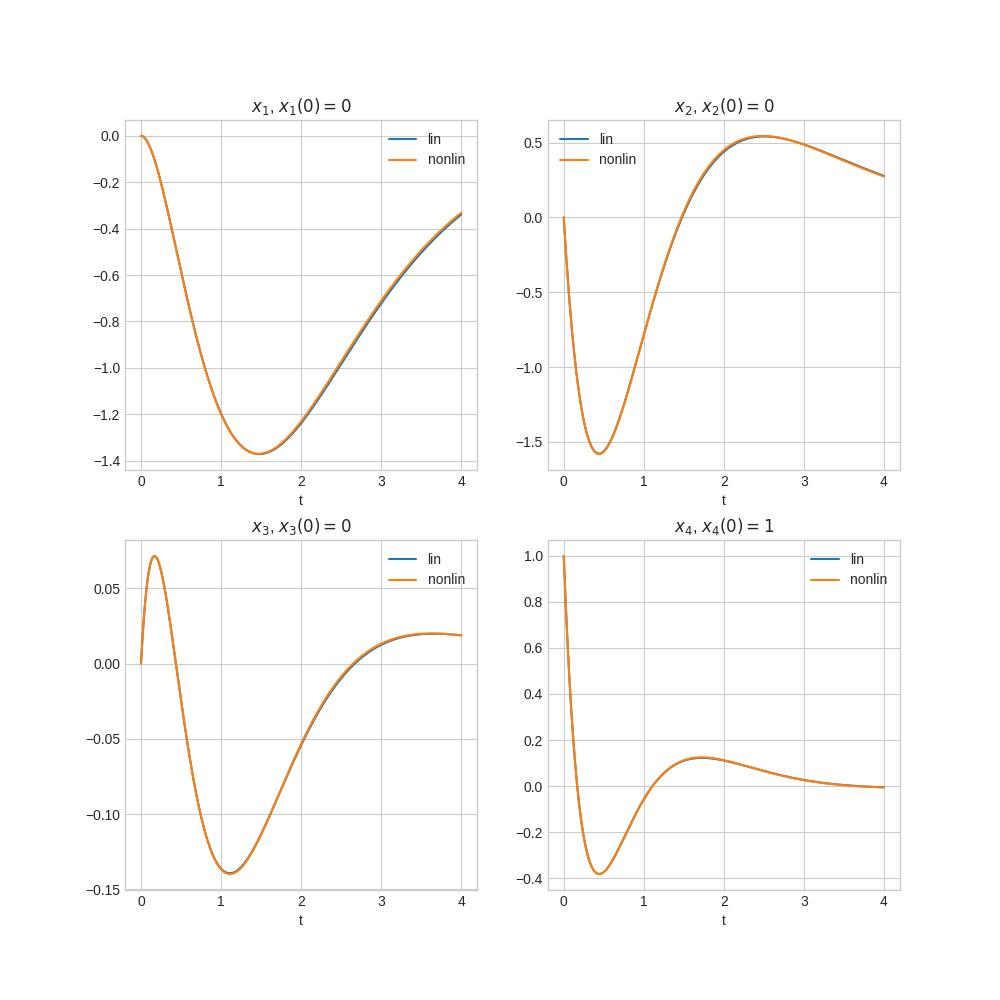
\includegraphics[width=\textwidth]{task3_1_0_0_0_1.jpg}
  \caption{Задание 3.1. Динамика системы.}
  \label{fig:task3_1_0_0_0_1.jpg}
\end{figure}
\begin{figure}[]
    \centering
    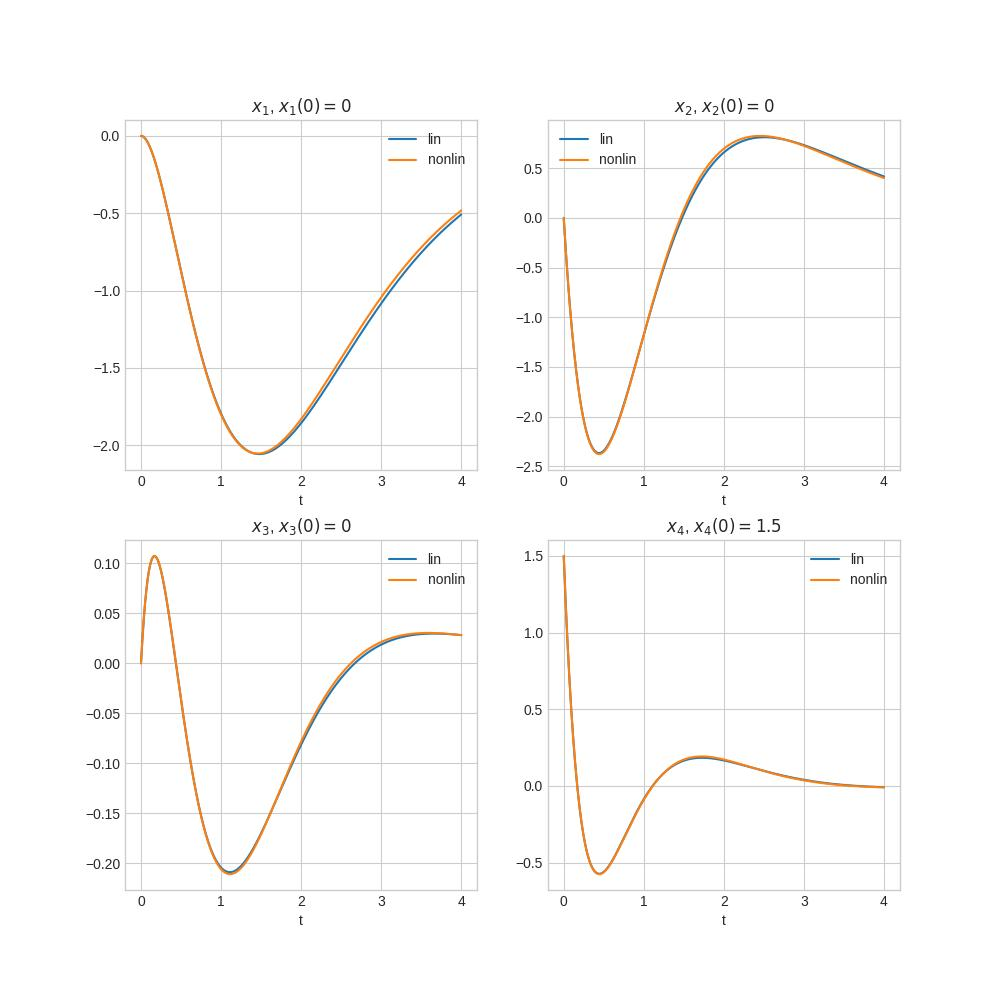
\includegraphics[width=\textwidth]{task3_1_0_0_0_1.5.jpg}
    \caption{Задание 3.1. Динамика системы.}
    \label{fig:task3_1_0_0_0_1.5.jpg}
  \end{figure}
  \begin{figure}[]
    \centering
    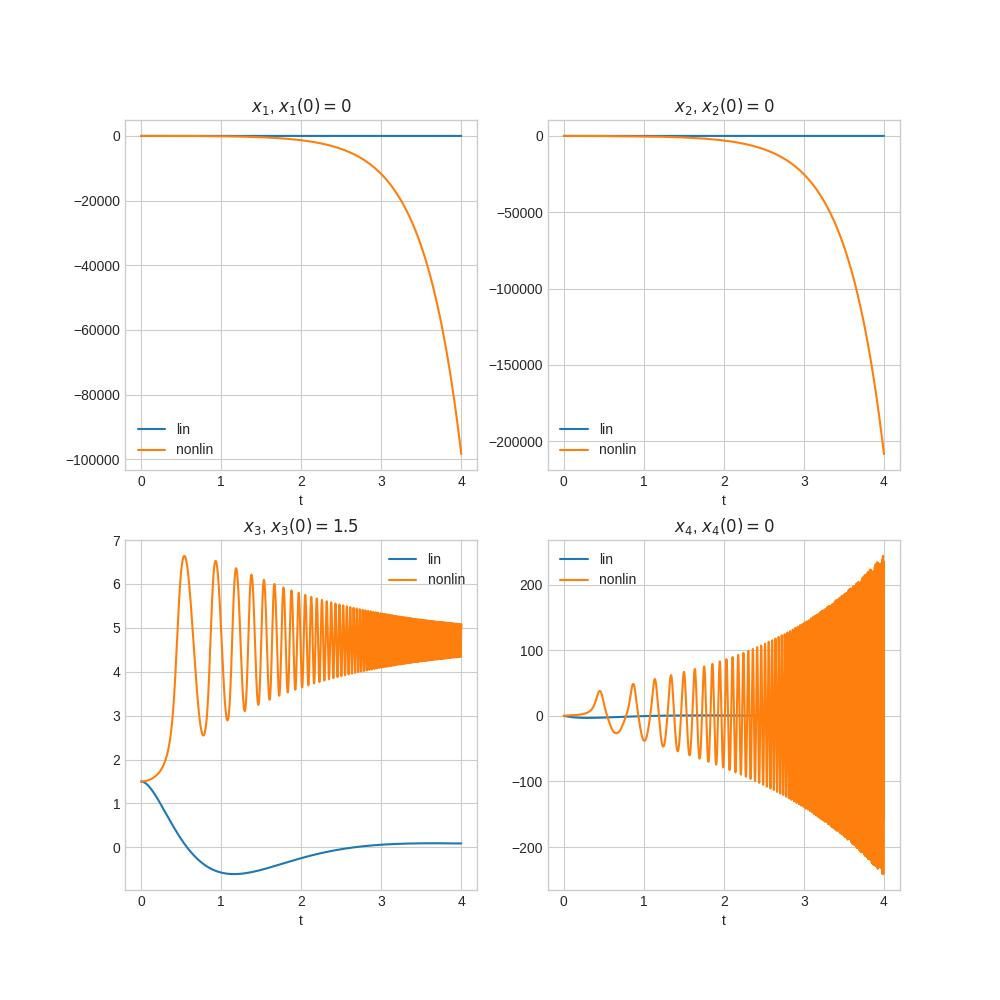
\includegraphics[width=\textwidth]{task3_1_0_0_1.5_0.jpg}
    \caption{Задание 3.1. Динамика системы.}
    \label{fig:task3_1_0_0_0_1.5.jpg}
  \end{figure}

\subsection{Исследование регулятора по состоянию}
\begin{center}
    \begin{tabular}{ c | c | c | c }
$\sigma G$ & $\max x$ & $\max \varphi$ & $\max u$ \\
        $\begin{bmatrix}
 -1.00 & -2.00 & -1.50 & -2.50
\end{bmatrix}$ & 7.4 & 2.7 & 293.0 \\
        $\begin{bmatrix}
 -0.10 & -0.20 & -0.15 & -0.25
\end{bmatrix}$ & 115.7 & 13.1 & 723.0 \\
        $\begin{bmatrix}
 -1.00 + 1.00j & -1.00 + -1.00j & -2.00 + 2.00j & -2.00 + -2.00j
\end{bmatrix}$ & 34887.2 & 201.4 & 2938438.6 \\
    \end{tabular}
\end{center}
В зависимости от спектра меняется возможность регулятора стабилизировать систему.
\subsection{Синтез наблюдателя}
Рассмотрим систему наблюдателя:
\begin{equation}
    \begin{cases}
        \dot{x} = A x \\
        y = C x \\
        \dot{\hat{x}} = A \hat{x} + L(\hat{y} - y) \\
        \hat{y} = C \hat{x}
\end{cases} 
\end{equation}



Для синтеза наблюдателя подбирается матрица \(\Gamma \in \mathbb{R}^{n \times n}\) с желаемым спектром и матрица \(Y \in \mathbb{R}^{n \times k}\), такая что пара \((\Gamma, Y)\) управляема.
\[L = \begin{bmatrix}
    7.65 &  19.64 & -292.95 & -89.64
  \end{bmatrix}\]
  \[\sigma(A + LC) = \begin{bmatrix}
    -2.50 & -2.00 & -1.50 & -1.00
\end{bmatrix}\]
На графиках видно, что не при любых начальных условиях наблюдатель сходится.

\begin{figure}[]
        \centering
        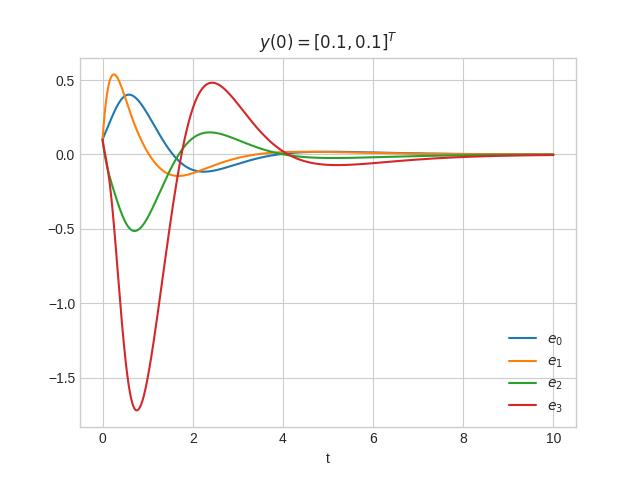
\includegraphics[width=\textwidth]{task3_3_0.1_0.1.jpg}
        \caption{Задание 3.3. Динамика ошибки.}
        \label{fig:task3_3_0.1_0.1.jpg}
\end{figure}
\begin{figure}[]
        \centering
        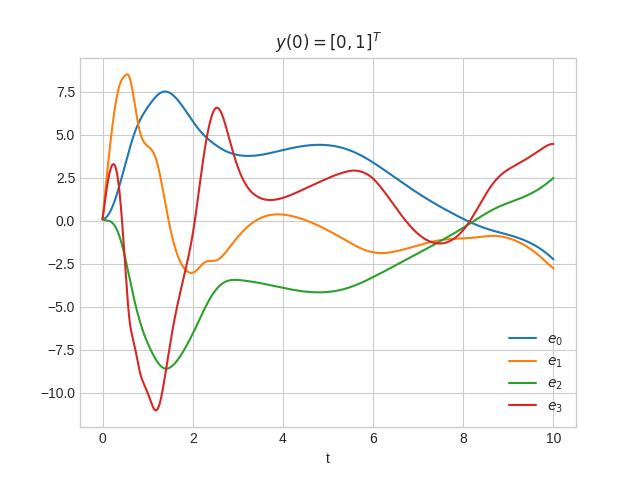
\includegraphics[width=\textwidth]{task3_3_0_1.jpg}
        \caption{Задание 3.3. Динамика ошибки.}
        \label{fig:task3_3_0_1.jpg}
\end{figure}

\begin{figure}[]
        \centering
        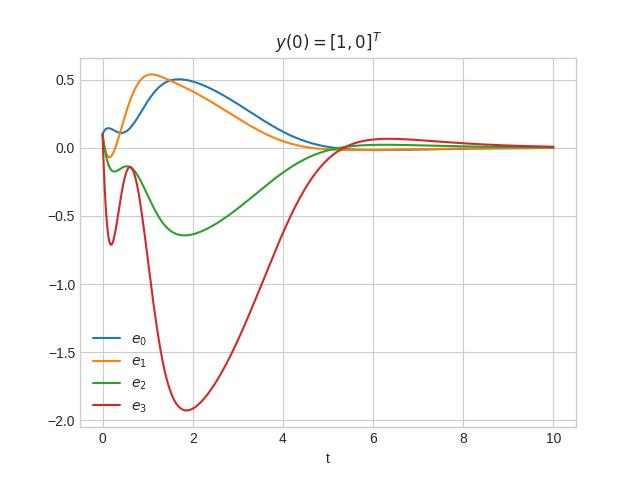
\includegraphics[width=\textwidth]{task3_3_1_0.jpg}
        \caption{Задание 3.3. Динамика ошибки.}
        \label{fig:task3_3_1_0.jpg}
\end{figure}


\subsection{Исследование наблюдателя}
Не при любом устойчивом спектре наблюдатель устойчив. 


\[L = \begin{bmatrix}
    7.65 &  19.64 & -292.95 & -89.64
  \end{bmatrix}\]
  \begin{figure}[]
    \centering
    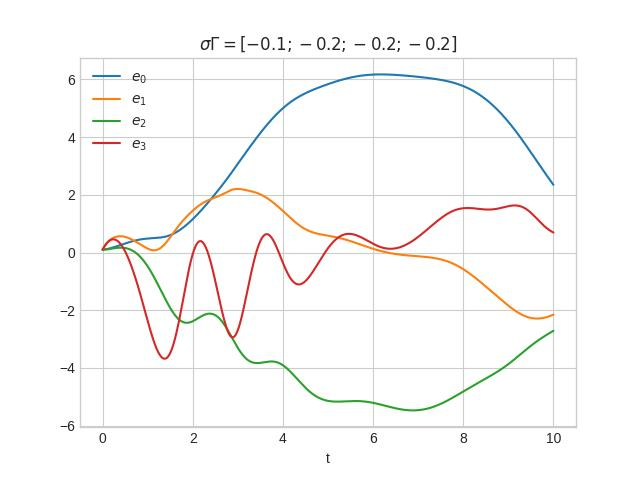
\includegraphics[width=\textwidth]{task3_4_-0.1_-0.2_-0.15_-0.25.jpg}
    \caption{Задание 3.4. Динамика ошибки.}
    \label{fig:task3_4_-0.1_-0.2_-0.15_-0.25.jpg}
\end{figure}

  \[\Gamma = diag(-1,-2,-1.5,-2.5)\]
  \[L = \begin{bmatrix}
    7.65 &  19.64 & -292.95 & -89.64
  \end{bmatrix}\]
  \begin{figure}[]
    \centering
    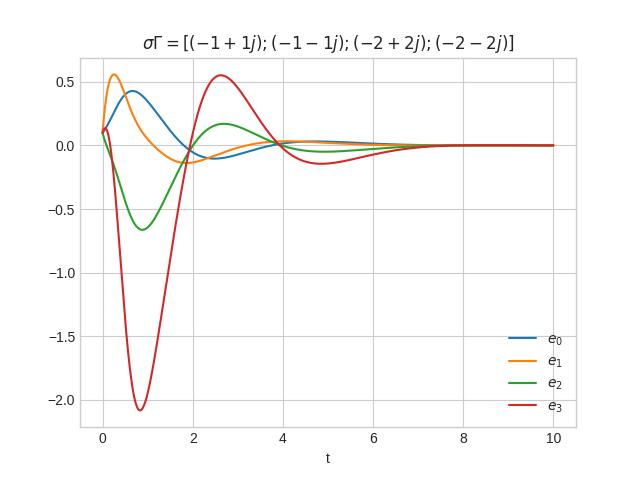
\includegraphics[width=\textwidth]{task3_4_(-1+1j)_(-1-1j)_(-2+2.0000000000000004j)_(-2-2.0000000000000004j).jpg}
    \caption{Задание 3.4. Динамика ошибки.}
    \label{fig:task3_4_(-1+1j)_(-1-1j)_(-2+2.0000000000000004j)_(-2-2.0000000000000004j).jpg}
\end{figure}


  \[\Gamma = diag(-0.1,-0.2,-0.15,-0.25)\]
  \[L = \begin{bmatrix}
    7.65 &  19.64 & -292.95 & -89.64
  \end{bmatrix}\]
  \[\Gamma = diag(-1\pm j, -2\pm j)\]
  \begin{figure}[]
    \centering
    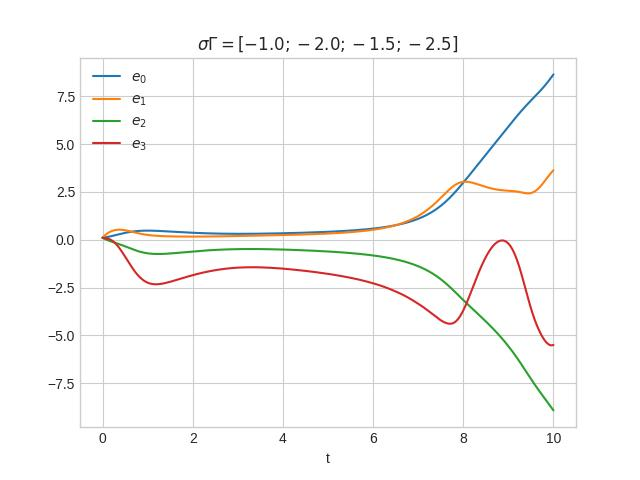
\includegraphics[width=\textwidth]{task3_4_-1.0_-2.0_-1.5_-2.5.jpg}
    \caption{Задание 3.4. Динамика ошибки.}
    \label{fig:task3_4_-1.0_-2.0_-1.5_-2.5.jpg}
\end{figure}

\subsection{Синтез регулятора по выходу}
На основе двух предыдущих пунктов получен регулятор по выходу.
\[L = \begin{bmatrix}
    1.05 &  1.05\\
   -1.74 & -1.74\\
   -8.05 & -8.05\\
   -26.79 & -26.79
  \end{bmatrix}\]
  \[K = \begin{bmatrix}
    7.65 &  19.64 & -292.95 & -89.64
  \end{bmatrix}\]
  \[\Gamma = \begin{bmatrix}
   -1.00 & -1.00 &  0.00 &  0.00\\
    1.00 & -1.00 &  0.00 &  0.00\\
    0.00 &  0.00 & -2.00 & -2.00\\
    0.00 &  0.00 &  2.00 & -2.00
  \end{bmatrix}\]

      \begin{figure}
        \centering
        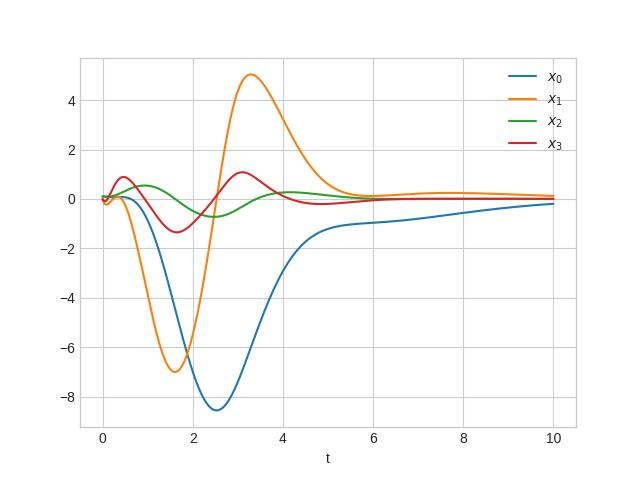
\includegraphics[width=\textwidth]{task3_5_0.1_0.0_0.1_0.0.jpg}
        \caption{Задание 3.5. Динамика компонент системы.}
        \label{fig:task3_5.jpg}
\end{figure}



\section{Регуляторы с заданной степенью устойчивости}

\subsection{Синтез регулятора по состоянию}
По сути, целью данного регулятора является изменение управляемых собственных чисел так, чтобы \(\forall \lambda \in \sigma(A): Re{\lambda} \leq \alpha\), где \(\alpha\) -- степень устойчивости.
Для этого используется LMI критерий экспоненциальной устойчивости:
\[ \exists Q \succ 0 , \alpha > 0 :  A^TQ + QA + 2 \alpha Q \preccurlyeq 0 \rightarrow
\begin{cases}
    \text{\(\forall x(0)\) А ассимптотически устойчива}\\
    \exists c :  ||x(t)|| \le  c e^{-\alpha t} ||x(0)|| \\
\end{cases}
\]
Для синтеза регулятора с заданной степенью устойчивости $\alpha$ необходимо найти матрицы $P$ и $Y$,
удовлетворяющие неравенствам:
\begin{equation}
    P \succ 0, PA^T + AP +2\alpha P + Y^TB^T + BY \prec 0
\end{equation}
Затем, получим матрицу $K$:
\begin{equation}
    K = YP^{-1}
\end{equation}

На практике, довольно часто \(P\) -- необратима. Приходится использовать псевдообратную.

\[\alpha = 1\]
\[K = \begin{bmatrix}
    95.12 &  114.09 & -732.81 & -172.27
  \end{bmatrix}\]
  \[spec(A + B K) = \begin{bmatrix}
   -1.68 + 6.30j & -1.68 + -6.30j & -1.23 + 0.83j & -1.23 + -0.83j
  \end{bmatrix}\]

  Иногда устойчивость линейной системы нарушается
  \begin{figure}[]
    \centering
    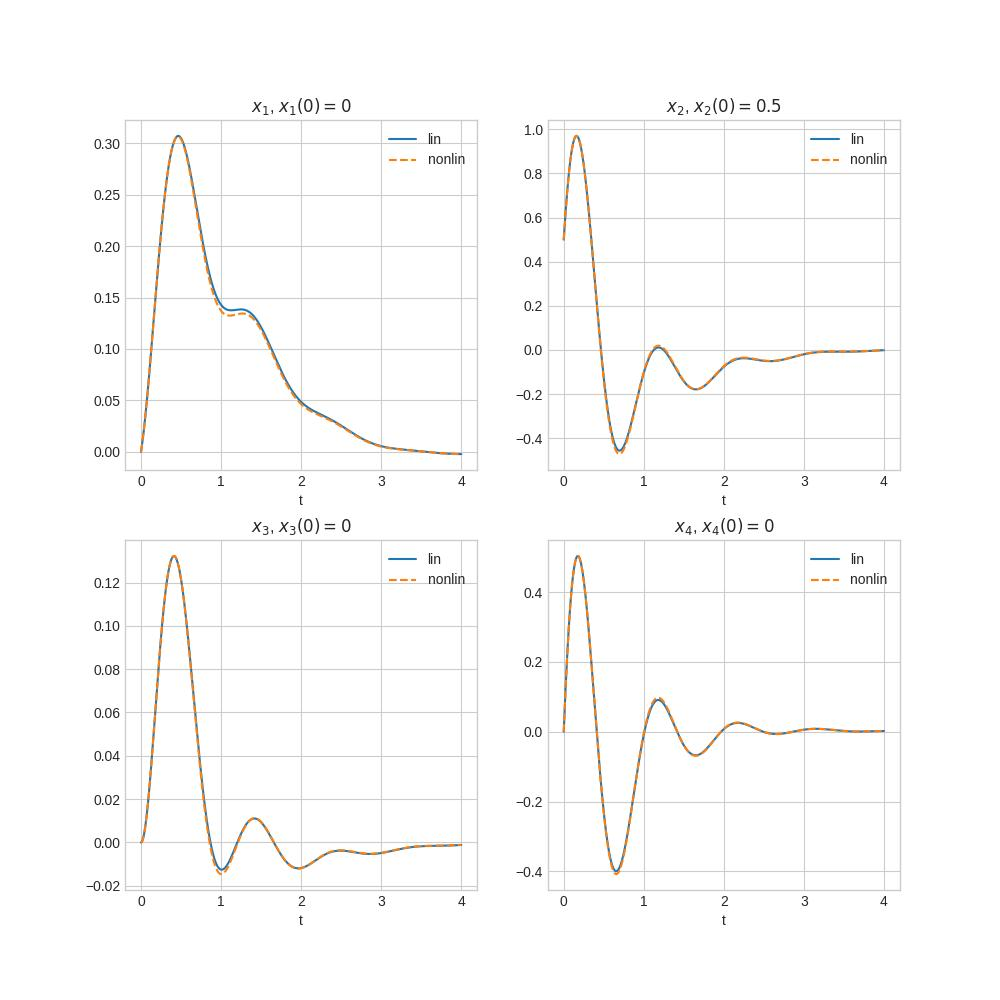
\includegraphics[width=\textwidth]{task4_1_0_0.5_0_0.jpg}
    \caption{Задание 4.1. Динамика системы.}
    \label{fig:task4_1_1}
\end{figure}

\begin{figure}[]
    \centering
    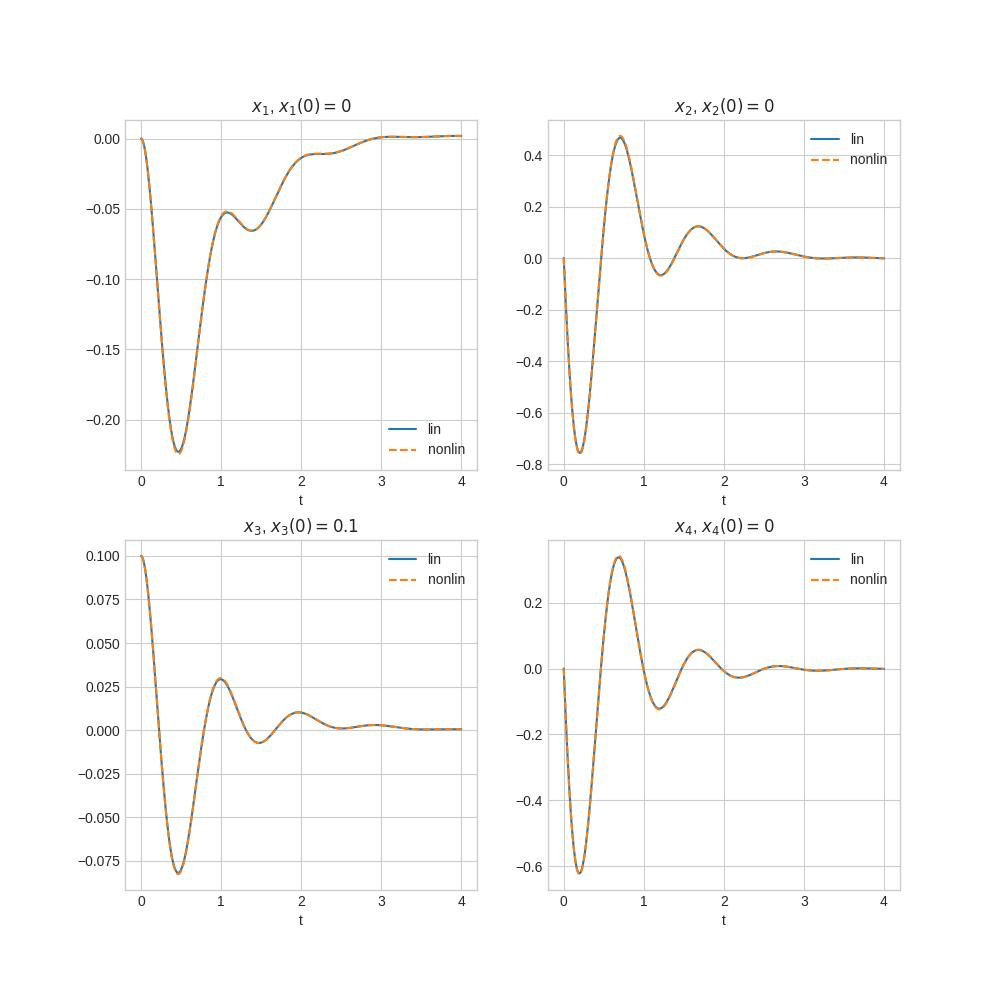
\includegraphics[width=\textwidth]{task4_1_0_0_0.1_0.jpg}
    \caption{Задание 4.1. Динамика системы.}
    \label{fig:task4_1_2}
\end{figure}

\begin{figure}[]
    \centering
    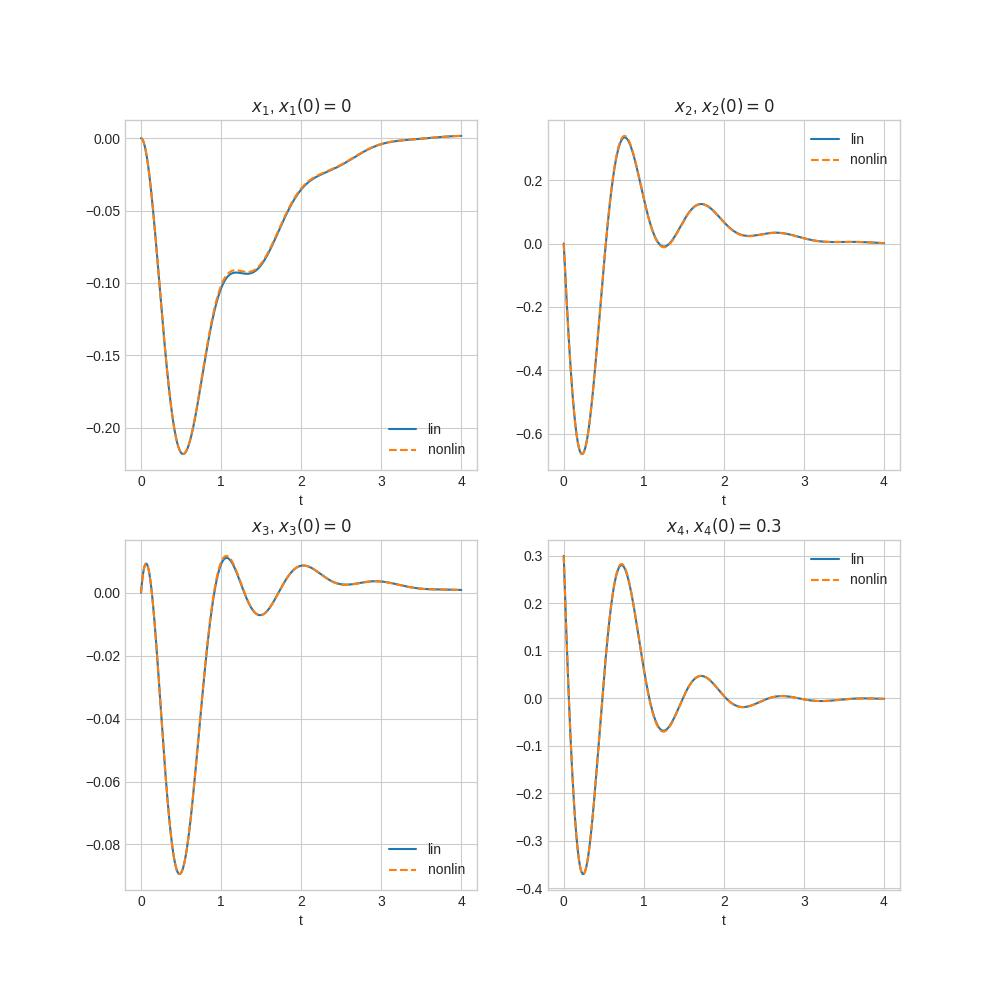
\includegraphics[width=\textwidth]{task4_1_0_0_0_0.3.jpg}
    \caption{Задание 4.1. Динамика системы.}
    \label{fig:task4_1_3}
\end{figure}

\begin{figure}[]
    \centering
    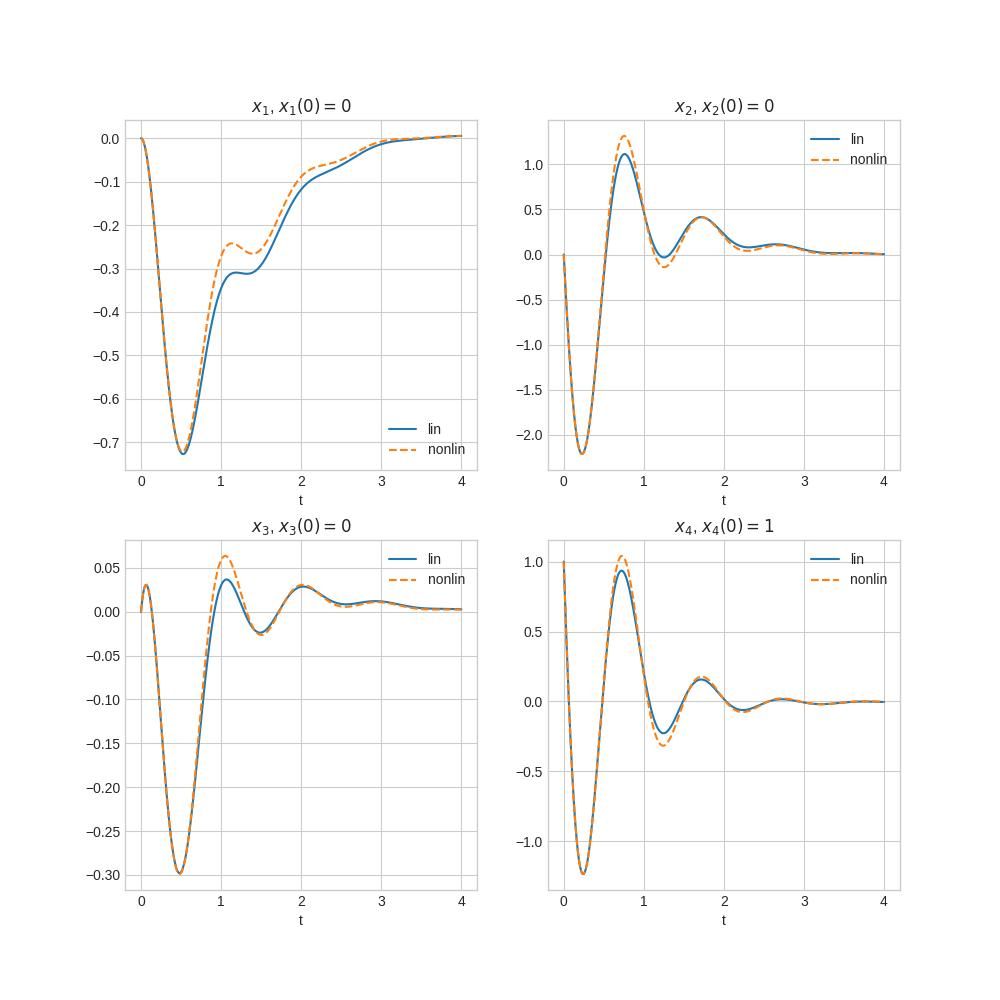
\includegraphics[width=\textwidth]{task4_1_0_0_0_1.jpg}
    \caption{Задание 4.1. Динамика системы.}
    \label{fig:task4_1_4}
\end{figure}

\begin{figure}[]
    \centering
    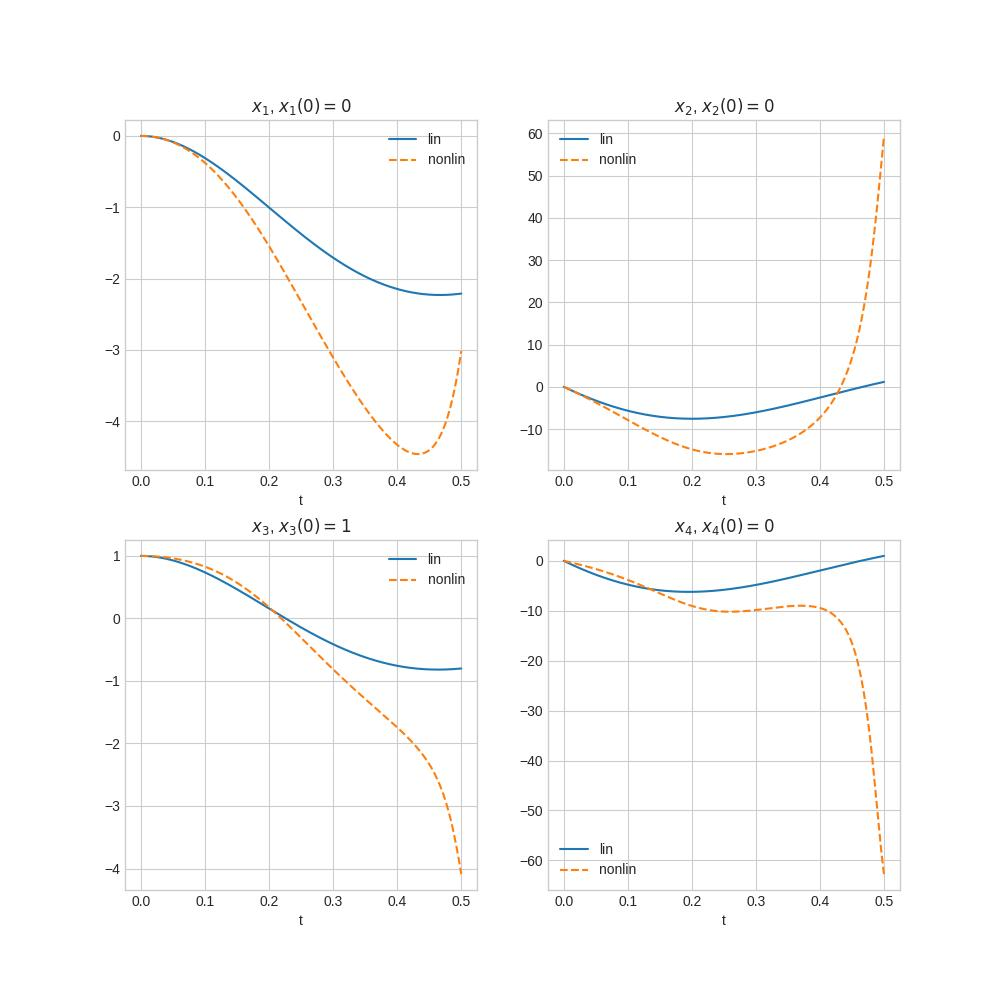
\includegraphics[width=\textwidth]{task4_1_0_0_1_0.jpg}
    \caption{Задание 4.1. Динамика системы.}
    \label{fig:task4_1_5}
\end{figure}

\begin{figure}[]
    \centering
    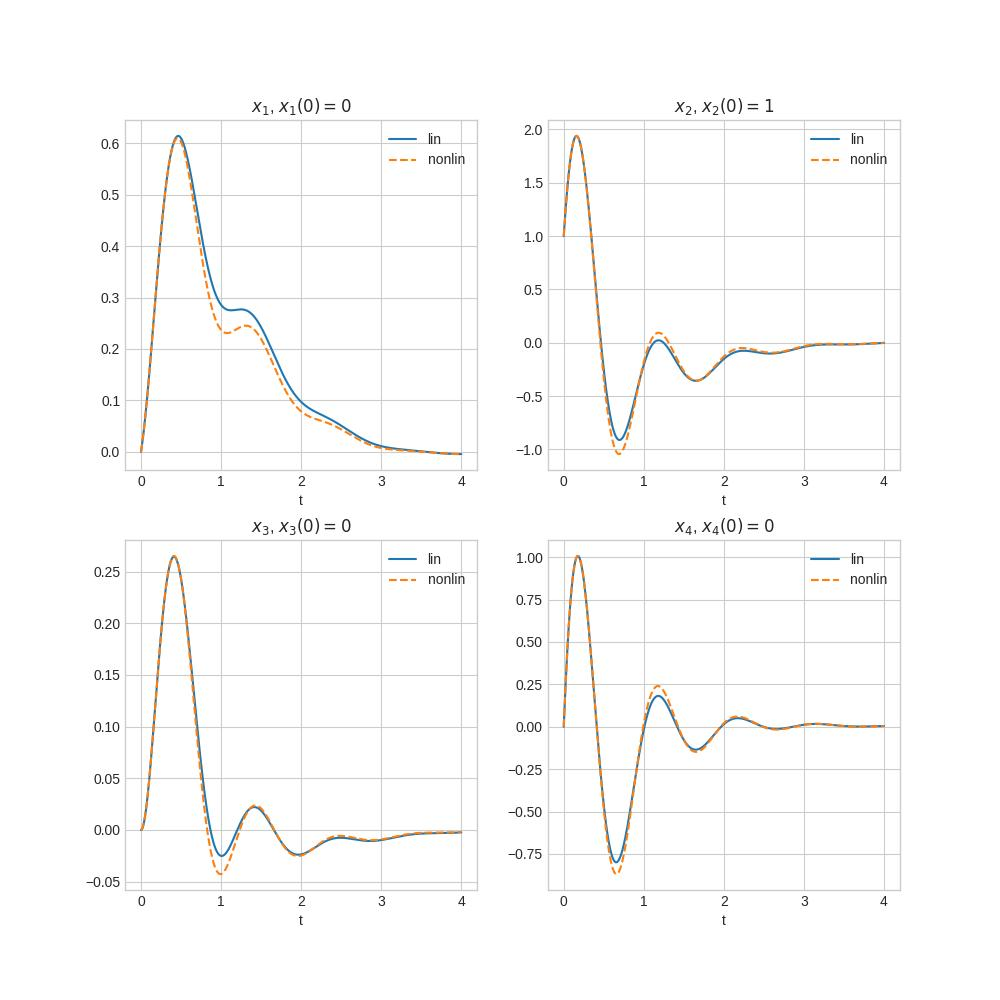
\includegraphics[width=\textwidth]{task4_1_0_1_0_0.jpg}
    \caption{Задание 4.1. Динамика системы.}
    \label{fig:task4_1_6}
\end{figure}



\subsection{Исследование регулятора по состоянию}
Ниже приведена таблица сравнений при \(x(0) = [0, 0, 0.1, 0]^T\). Приведено поведение системы при различных начальных условиях.
\begin{center}
    \begin{tabular}{ c | c c c }
$\alpha$ & $\max x$ & $\max \varphi$ & $\max u$ \\
        $0.1$ & 0.27 & 0.1 & 20.1 \\
        $0.8$ & 0.24 & 0.1 & 35.5 \\
        $1.5$ & 0.21 & 0.1 & 40.7 \\
    \end{tabular}
\end{center}

\begin{figure}[]
    \centering
    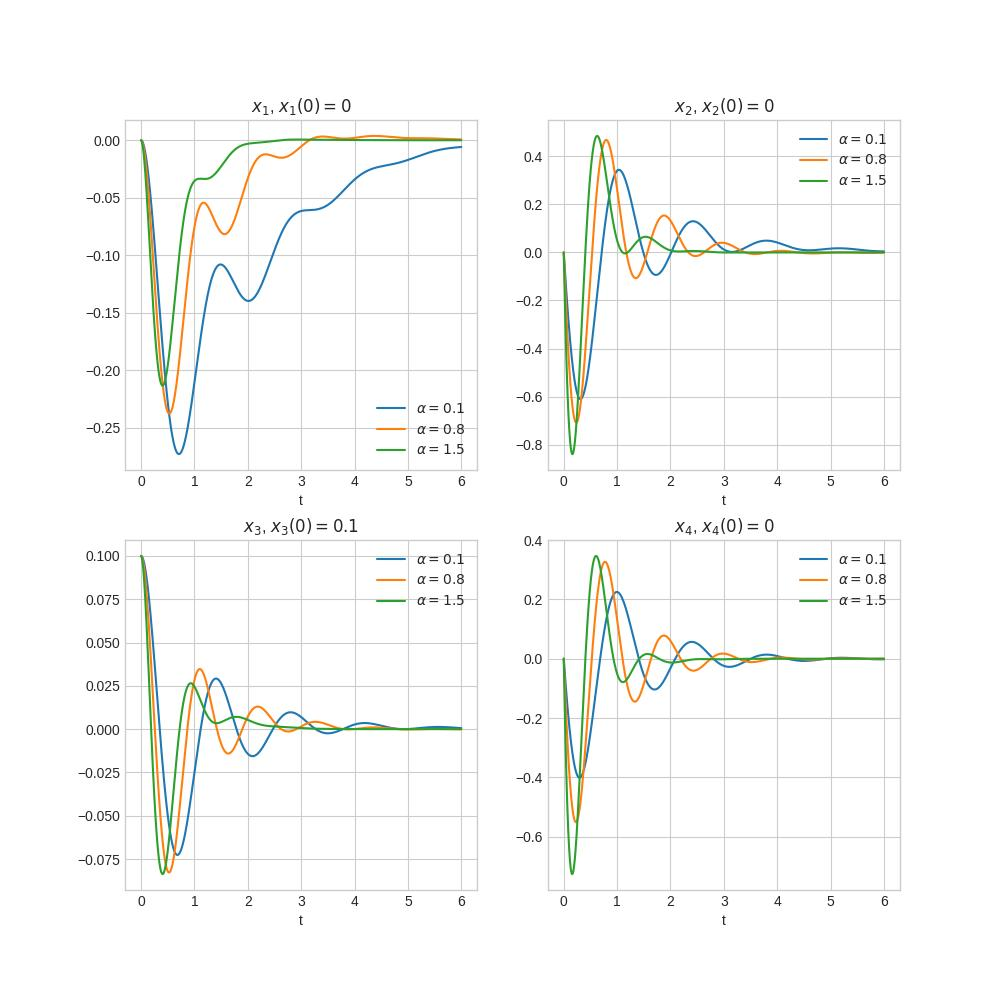
\includegraphics[width=\textwidth]{task4_2_0_0_0.1_0.jpg}
    \caption{Задание 4.2. Динамика системы.}
    \label{fig:task4_2_1}
\end{figure}
\begin{figure}[]
    \centering
    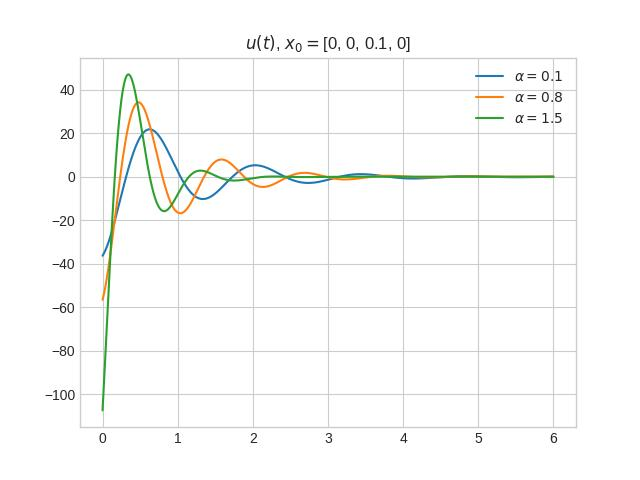
\includegraphics[width=\textwidth]{task4_2_u_0_0_0.1_0.jpg}
    \caption{Задание 4.2. Динамика воздействия.}
    \label{fig:task4_2_2}
\end{figure}


\subsection{Синтез регулятора по состоянию с ограничением на управление}

В этом задании выводится ограничение на управление \(||u(t)|| \leq \mu\). Тогда система уравнений принимает вид: 
\[
        \begin{cases}
                \begin{bmatrix}
                    P &  x_0\\
                    x_0^T &  1 \\
                \end{bmatrix} \succ 0 \\
                \\
                \begin{bmatrix}
                    P &  Y^T\\
                    Y &  \mu^2I \\
                \end{bmatrix} \succ 0 \\
                P \succ 0 \\
                PA^T + AP + 2 \alpha P + Y^T B^T + BY \preccurlyeq 0  \\
                K = YP^{-1}\\
        \end{cases} 
\]
\begin{figure}[]
    \centering
    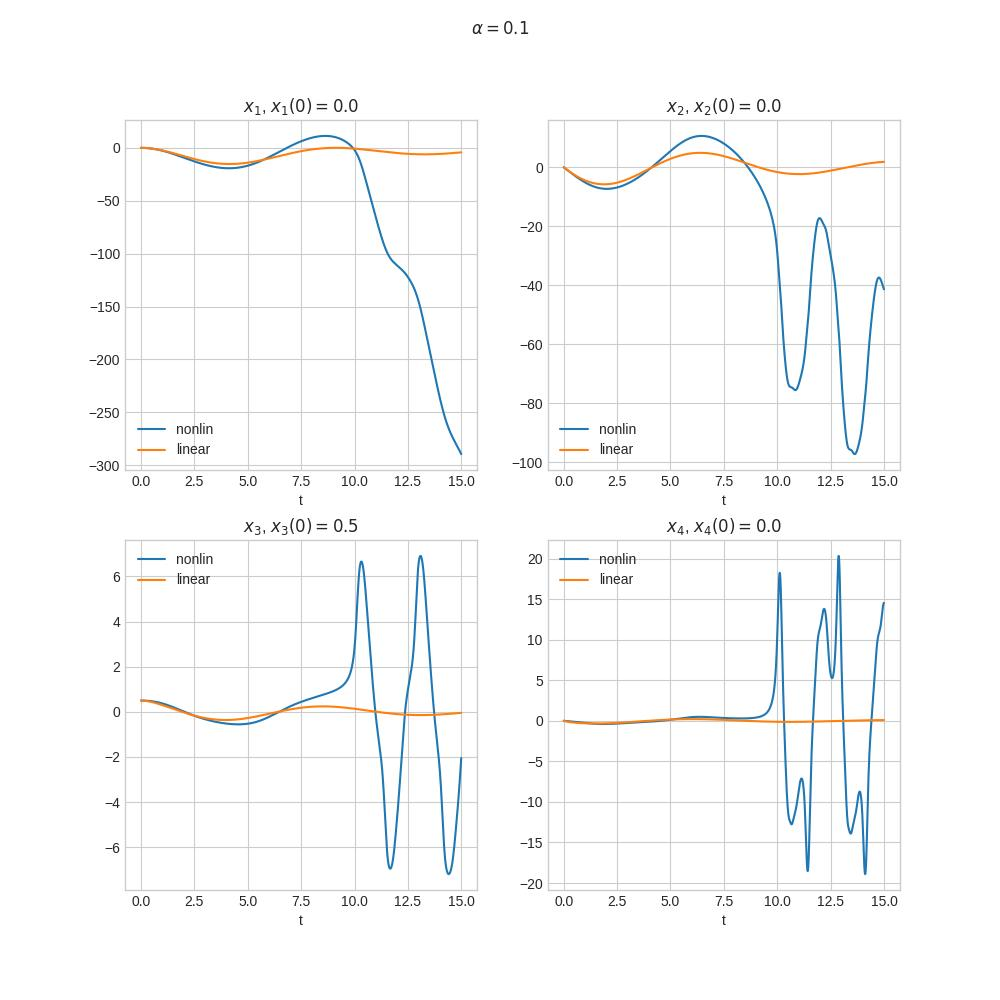
\includegraphics[width=\textwidth]{task4_3_0.1.jpg}
    \caption{Задание 4.3. Динамика системы}
    \label{fig:task4_3_0.1}
\end{figure}
\begin{figure}[]
    \centering
    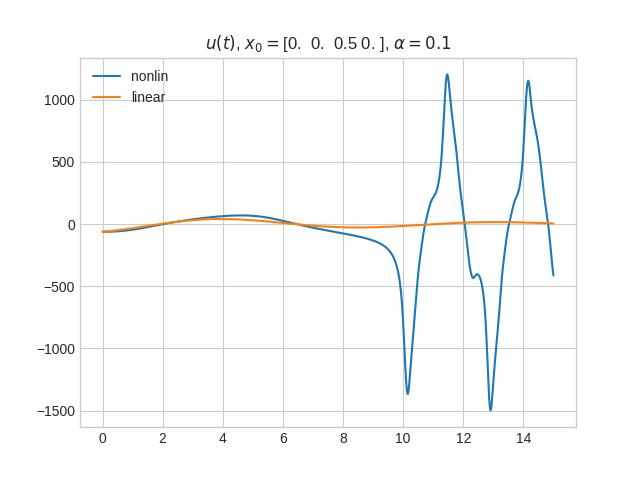
\includegraphics[width=\textwidth]{task4_3_u_0.1.jpg}
    \caption{Задание 4.3. Динамика воздействия}
    \label{fig:task4_3_u_0.1}
\end{figure}

\begin{figure}[]
    \centering
    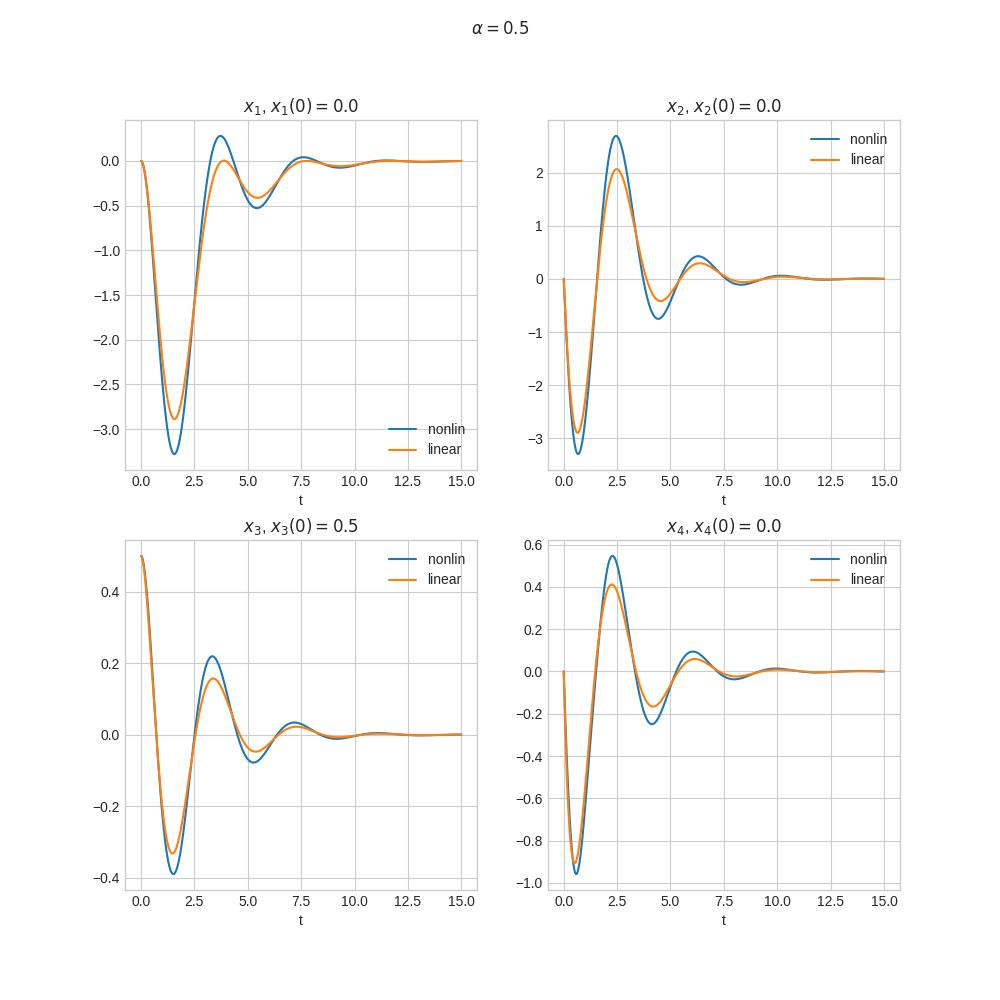
\includegraphics[width=\textwidth]{task4_3_0.5.jpg}
    \caption{Задание 4.3. Динамика системы}
    \label{fig:task4_3_0.5}
\end{figure}
\begin{figure}[]
    \centering
    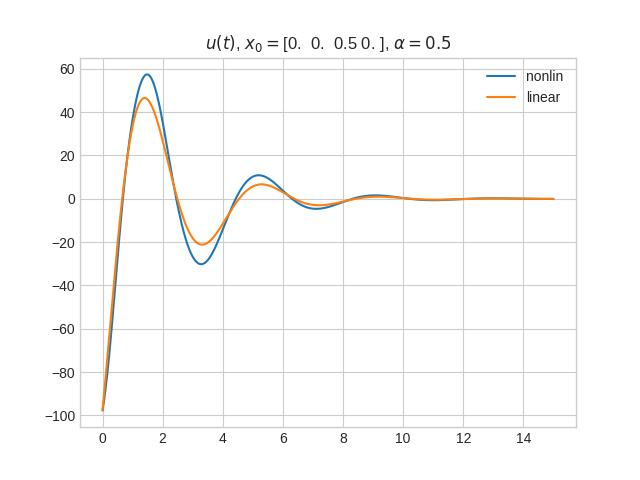
\includegraphics[width=\textwidth]{task4_3_u_0.5.jpg}
    \caption{Задание 4.3. Динамика воздействия}
    \label{fig:task4_3_u_0.5}
\end{figure}

\begin{figure}[]
    \centering
    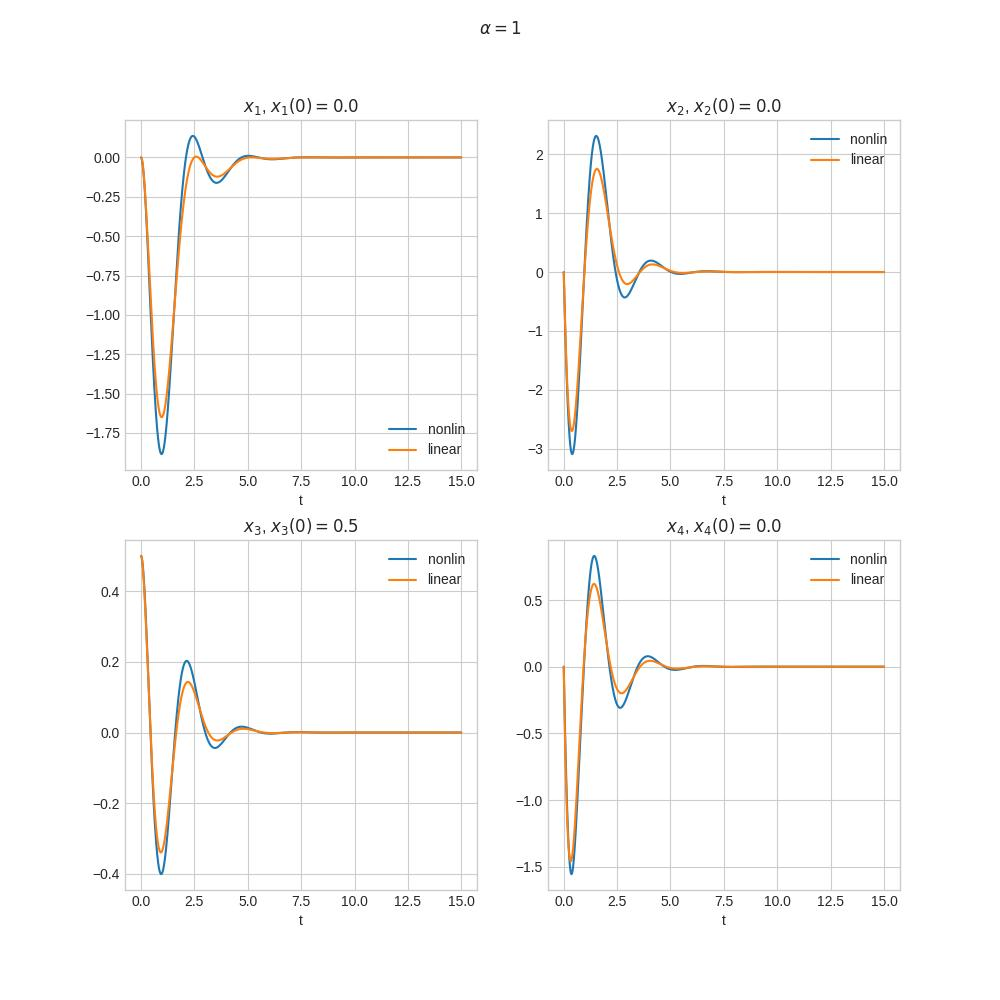
\includegraphics[width=\textwidth]{task4_3_1.jpg}
    \caption{Задание 4.3. Динамика системы}
    \label{fig:task4_3_1}
\end{figure}
\begin{figure}[]
    \centering
    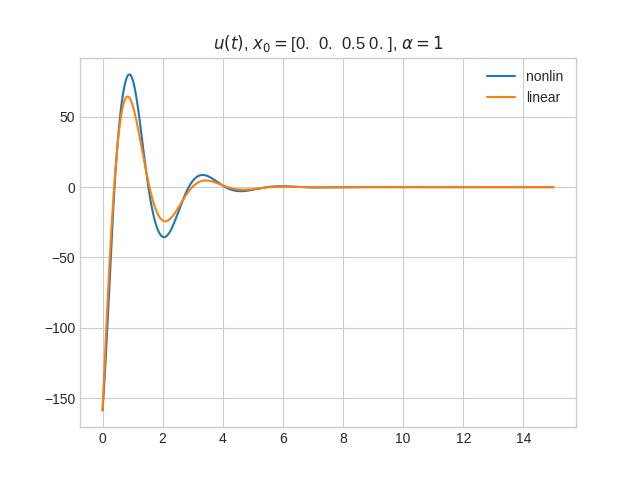
\includegraphics[width=\textwidth]{task4_3_u_1.jpg}
    \caption{Задание 4.3. Динамика воздействия}
    \label{fig:task4_3_u_1}
\end{figure}


\subsection{Синтез наблюдателя}

В этом задании выводится наблюдатель заданной степени устойчивости для системы:
\[
        \begin{cases}
                \dot{x} = A x \\
                y = C x \\
                \dot{\hat{x}} = A \hat{x} + L(\hat{y} - y) \\
                \hat{y} = C \hat{x}
        \end{cases} 
\]

Для этого достаточно решить систему:
\[
        \begin{cases}
                L = Q^{-1}Y\\
                Q \succ 0 \\
                A^TQ + QA + 2 \alpha Q + C^T Y^T + YC \preccurlyeq 0  \\
        \end{cases} 
\]
\[ \alpha = 1\]
\[L = \begin{bmatrix}
 -4.48 & -0.63\\
 -8.92 & -2.11\\
  0.63 & -4.48\\
  1.11 & -19.92
\end{bmatrix}\]
\[spec(A + LC) = \begin{bmatrix}
 -2.31 + 2.32j & -2.31 + -2.32j & -2.17 + 1.69j & -2.17 + -1.69j
\end{bmatrix}\]
\begin{figure}[]
    \centering
    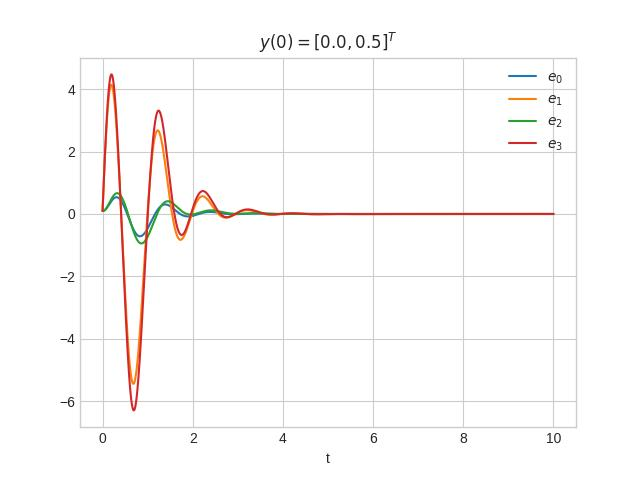
\includegraphics[width=\textwidth]{task4_4_0.0_0.5.jpg}
    \caption{Задание 4.4. Динамика ошибки наблюдателя}
    \label{fig:task4_4_1}
\end{figure}

\begin{figure}[]
    \centering
    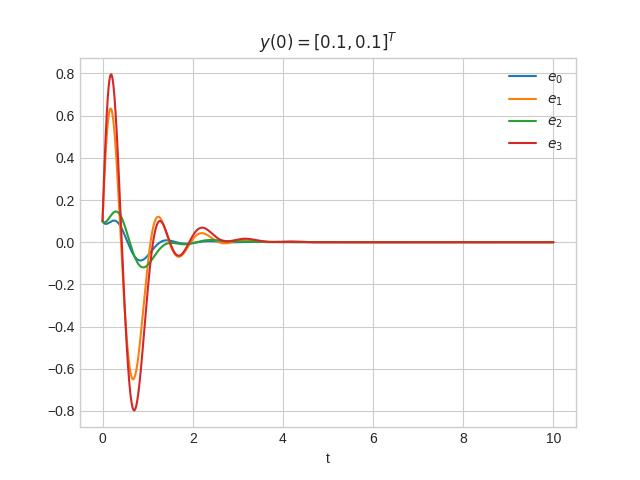
\includegraphics[width=\textwidth]{task4_4_0.1_0.1.jpg}
    \caption{Задание 4.4. Динамика ошибки наблюдателя}
    \label{fig:task4_4_2}
\end{figure}

\begin{figure}[]
    \centering
    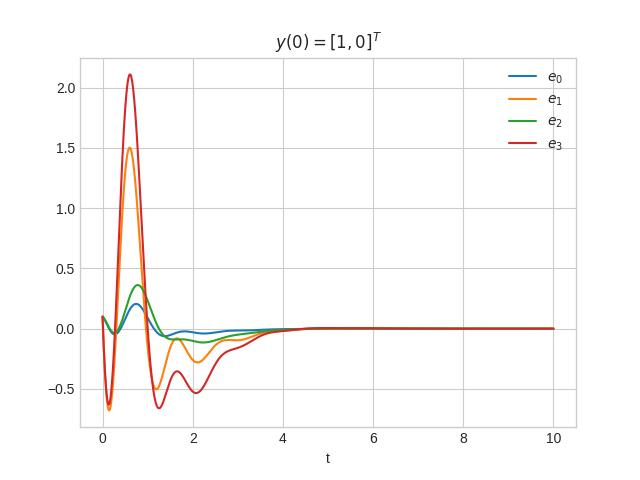
\includegraphics[width=\textwidth]{task4_4_1_0.jpg}
    \caption{Задание 4.4. Динамика ошибки наблюдателя}
    \label{fig:task4_4_3}
\end{figure}


\subsection{Синтез регулятора по выходу}
В этом задании выводится наблюдатель регулятор для системы. Так бы это выглядело для линейной системы.
\[
        \begin{cases}
                \dot{x} = A x + B u\\
                y = C x \\
                \dot{\hat{x}} = A \hat{x} + B u + L(\hat{y} - y) \\
                \hat{y} = C \hat{x} \\
                u = K \hat{x}
        \end{cases} \rightarrow
        \begin{cases}
            \begin{bmatrix} 
                \dot{x} \\
                \dot{e}
            \end{bmatrix} = 
            \begin{bmatrix} 
                A + BK & -BK\\
                0 & A + LC
            \end{bmatrix}
            \begin{bmatrix} 
              x \\
              e
          \end{bmatrix} 
            \\
            \hat{x} = x - e \\
            y = Cx \\
            \hat{y} = C \hat{x}
         \end{cases}
\]

Удалось стабилизировать нелинейную систему.
\begin{figure}[]
    \centering
    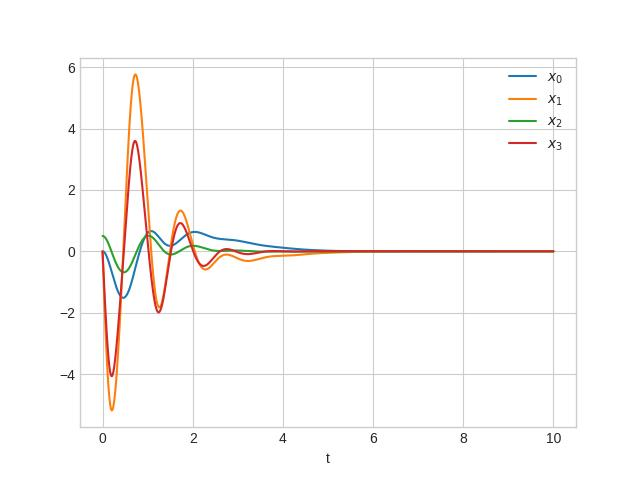
\includegraphics[width=\textwidth]{task4_5_0.0_0.0_0.5_0.0.jpg}
    \caption{Задание 4.5. Динамика системы}
    \label{fig:task4_5}
\end{figure}


\section{LQR \& фильтр Калмана}
\subsection{Синтез линейно-квадратичного регулятора}
LQR позволяет оптимизировать критерий качества:
\[J = \int_0^\infty (x^T Q x + u^T R u)dt \]
Выбор cотношения матриц \(Q\) и \(R\) позволяет управлять временем сходимости и величиной подаваего управления: чем больше \(\frac{Q}{R}\), тем больше управление и быстрее сходимость.

\(K\) получается решением следующих уравнений:
    \begin{equation}
        \begin{cases}
            A^T P + P A + Q - PBR^{-1}B^TP = 0\\
            K = -R^{-1} B^T P \\
        \end{cases}
    \end{equation}

Теоретический минимум критерия качества:
\[J_{min} = x_0^T P x_0\]
В следующих заданиях применим регулятор для стабилизации системы.

\subsection{Исследование линейно-квадратичного регулятора}
Проведем исследование при разных матрицах (графики ниже):
\[Q = 0.1; R = 10.0; K_0 = \begin{bmatrix}
    -0.10 & -1.55 &  224.67 &  68.57
   \end{bmatrix}\]
   \[\sigma(A+BK_0) = \begin{bmatrix}
    -0.07 + 0.07j & -0.07 + -0.07j & -3.29 + 0.00j & -3.28 + 0.00j
   \end{bmatrix}\]
   \[Q = 1.0; R = 1.0; K_1 = \begin{bmatrix}
    -1.00 & -5.41 &  246.16 &  75.45
   \end{bmatrix}\]
   \[\sigma(A+BK_1) = \begin{bmatrix}
    -0.22 + 0.21j & -0.22 + -0.21j & -3.33 + 0.00j & -3.24 + 0.00j
   \end{bmatrix}\]
   \[Q = 10.0; R = 0.1; K_2 = \begin{bmatrix}
    -10.00 & -24.11 &  343.62 &  107.01
   \end{bmatrix}\]
   \[\sigma(A+BK_2) = \begin{bmatrix}
    -3.83 + 0.00j & -2.84 + 0.00j & -0.81 + 0.50j & -0.81 + -0.50j
   \end{bmatrix}\]

\begin{figure}[]
        \centering
        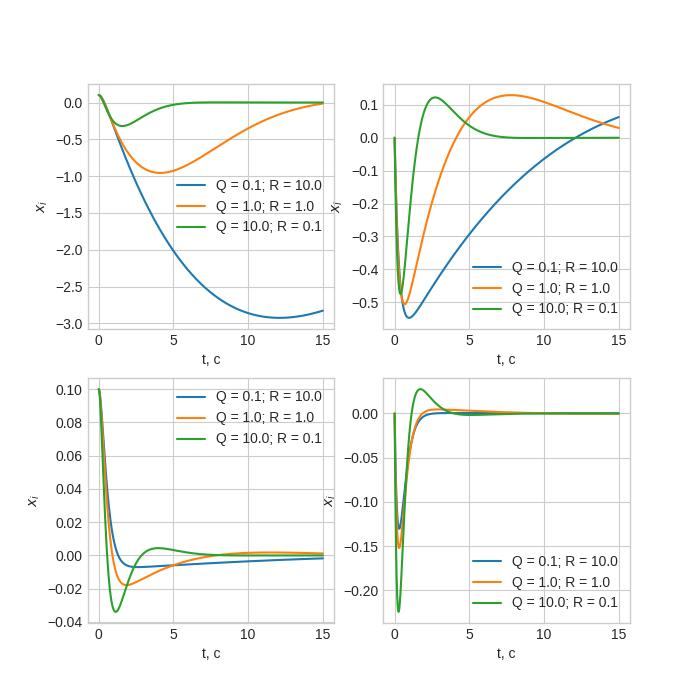
\includegraphics[width=\textwidth]{task5_states.jpg}
        \caption{Задание 5.2. Динамика компонент системы.}
        \label{fig:task5_states}
\end{figure}

\begin{figure}[]
        \centering
        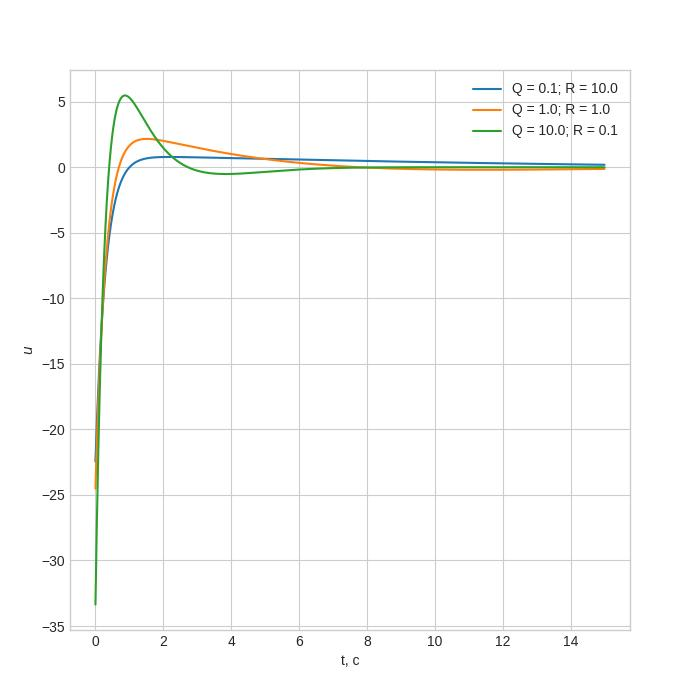
\includegraphics[width=\textwidth]{task5_us.jpg}
        \caption{Задание 5.2. Управление.}
        \label{fig:task5_u}
\end{figure}


\subsection{Синтез фильтра Калмана}
\begin{equation}
    \dot{x} = Ax + f, y = Cx + \xi
\end{equation}
Внешние возмущения $f$ и $\xi$  будем считать белым шумам с заданной дисперсией.
Матрицы \(Q\) и \(R\) обозначают, насколько сильно мы оцениваем влияние \(f\) и \(\xi\).

\(L\) получается решением следующих уравнений:
\[
\begin{cases}
    A P + P A^T + Q - PC^TR^{-1}CP = 0\\
    L = -P C^T R^{-1}\\
\end{cases}
\]
\[Q = 0.01; R = 0.01; L = \begin{bmatrix}
    1.76 &  0.37\\
    1.11 &  1.84\\
    0.37 &  6.63\\
    1.23 &  21.54
  \end{bmatrix}\]
\begin{figure}[]
        \centering
        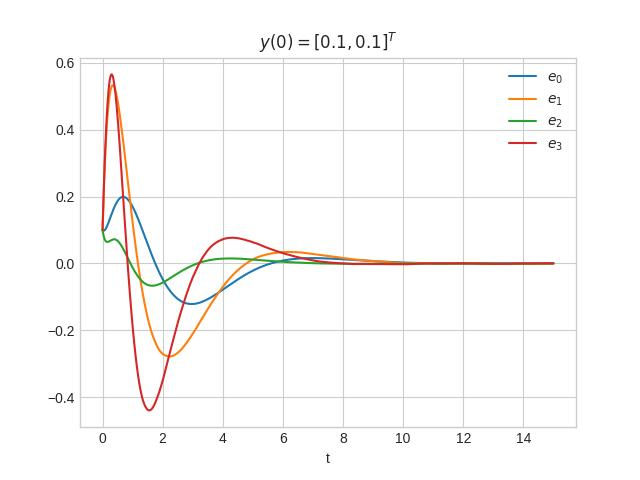
\includegraphics[width=\textwidth]{task5_3.jpg}
        \caption{Задание 5.3. Ошибка.}
        \label{fig:task5_3}
\end{figure}


\subsection{ LQG для линейной модели}
В этом задании выводится наблюдатель регулятор для системы:
\[
        \begin{cases}
                \dot{x} = A x + B  K \hat{x} + f \\
                y = Cx + DK\hat{x} + \xi \\
                \dot{\hat{x}} = A \hat{x} + B  K \hat{x} + L(\hat{y} - y) \\
                \hat{y} = C \hat{x} + D K \hat{x} \\
                \hat{x} = x - e \\
        \end{cases} \rightarrow
        \begin{cases}
            \begin{bmatrix} 
                \dot{x} \\
                \dot{e}
            \end{bmatrix} = 
            A_{new}
            \begin{bmatrix} 
              x \\
              e
            \end{bmatrix} 
          + B_{new} 
          \begin{bmatrix} 
            f \\
            \xi
          \end{bmatrix} 
            \\
            A_{new} = 
            \begin{bmatrix} 
                A + BK & -BK\\
                0 & A + LC
            \end{bmatrix} \\
            B_{new} = 
            \begin{bmatrix} 
                I & 0\\
                I & L
            \end{bmatrix} \in R^{2n \times (n + m)}
         \end{cases}
\]
\[Q = 0.01; R = 0.01; L = \begin{bmatrix}
        -1.76 & -0.37\\
        -1.11 & -1.88\\
        -0.37 & -6.69\\
        -1.26 & -21.97
       \end{bmatrix}\]
       \[spec(A+LC) = \begin{bmatrix}
        -0.87 + 0.50j & -0.87 + -0.50j & -2.88 + 0.00j & -3.84 + 0.00j
       \end{bmatrix}\]
       \[Q = 1; R = 1; K= \begin{bmatrix}
         1.00 &  2.40 & -34.91 & -10.76
       \end{bmatrix}\]
       \[spec(A + BK) = \begin{bmatrix}
        -3.86 + 0.00j & -2.87 + 0.00j & -0.81 + 0.50j & -0.81 + -0.50j
       \end{bmatrix}\]
\begin{figure}[]
        \centering
        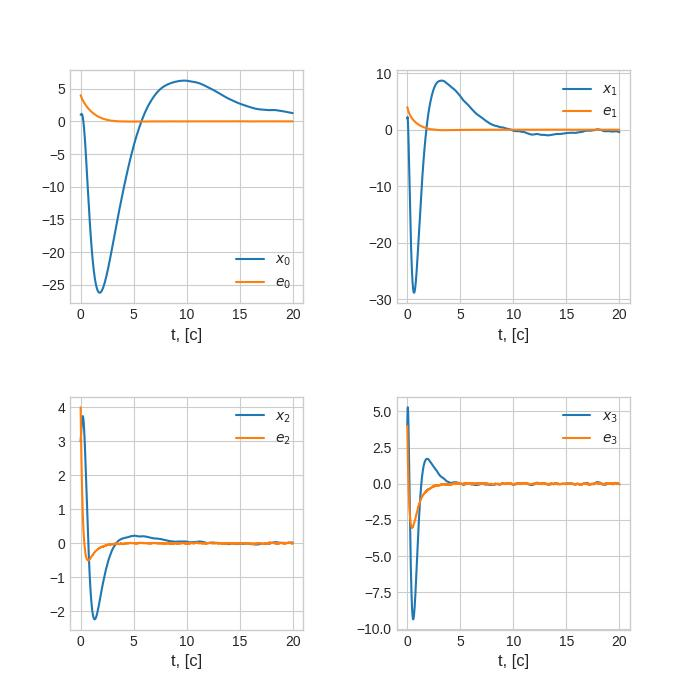
\includegraphics[width=\textwidth]{task5_LQG_lin.jpg}
        \caption{Задание 5.4. Динамика системы и ошибки.}
        \label{fig:task5_4}
\end{figure}


\subsection{ LQG для нелинейной модели}
\[Q = 0.01; R = 0.01; L = \begin{bmatrix}
        1.76 &  0.37\\
        1.11 &  1.88\\
        0.37 &  6.69\\
        1.26 &  21.97
      \end{bmatrix}\]
      \[Q = 0.01; R = 0.01; L = \begin{bmatrix}
       -1.76 & -0.37\\
       -1.11 & -1.88\\
       -0.37 & -6.69\\
       -1.26 & -21.97
      \end{bmatrix}\]
      \[spec(A+LC) = \begin{bmatrix}
       -0.87 + 0.50j & -0.87 + -0.50j & -2.88 + 0.00j & -3.84 + 0.00j
      \end{bmatrix}\]
      \[Q = 1; R = 1; K= \begin{bmatrix}
        1.00 &  2.40 & -34.91 & -10.76
      \end{bmatrix}\]
      \[spec(A + BK) = \begin{bmatrix}
       -3.86 + 0.00j & -2.87 + 0.00j & -0.81 + 0.50j & -0.81 + -0.50j
      \end{bmatrix}\]
\begin{figure}[]
        \centering
        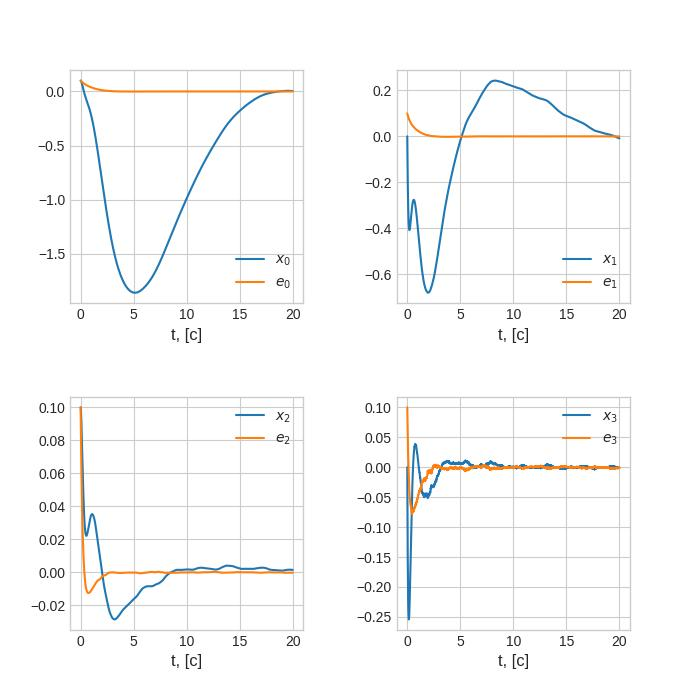
\includegraphics[width=\textwidth]{task5_LQG_non_lin.jpg}
        \caption{Задание 5.5. Динамика системы и ошибки.}
        \label{fig:task5_5}
\end{figure}
\pagebreak

\section{Слежение и компенсация}
\subsection{Компенсация}
Рассмотрим систему вида:
\begin{equation}
    \begin{cases}
        \dot{x} = A_1x + B_1u + B_2w \\
        z = C_2x
    \end{cases},
\end{equation}
где $w$:
\begin{equation}
    \dot{w} = A_2w
\end{equation}

Для данной системы можем синтезировать регулятор вида $u = K_1x + K_2w$, гарантирующий:
\begin{equation*}
    \lim_{t\to\infty} z(t) = 0
\end{equation*}

$K_1$ можем выбрать как матрицу регулятора, синтезированного любым способом (в данном случае модальное управление). Матрицу $K_2$ найдем следующим образом:
\begin{equation}
    \begin{cases}
        PA_2 - A_1P = B_1Y + B_2\\
        C_2P + D_2 = 0 \\
        K_2 = Y - K_1P
    \end{cases}
\end{equation}

\begin{equation*}
    A_2 = 
    \begin{bmatrix}
        0 & 2 & 0 & 0 \\
        -2 & 0 & 0 & 0 \\
        0 & 0 & 0 & 3 \\
        0 & 0 & -3 & 0
    \end{bmatrix},
    B_2 = 
    \begin{bmatrix}
        0 & 0 & 0 & 0 \\
        0 & 0.033 & 0.066 & 0.1 \\
        0 & 0 & 0 & 0 \\
        0 & 0.36 & 0.73 & 1.1 
    \end{bmatrix},
    D_2 - \text{нулевая},
    B_2w = Df
\end{equation*}
Проведем моделирование с нелинейной системой:
\begin{figure}[]
    \centering
    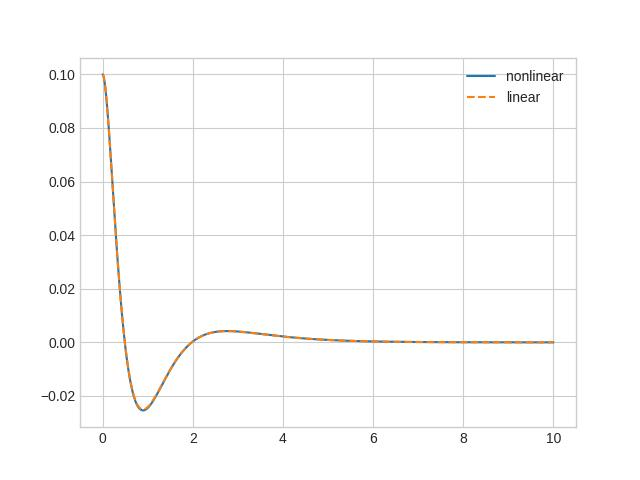
\includegraphics[width=\textwidth]{task6_1_0.1_0.0_0.1_0.0.jpg}
    \caption{Задание 6.1. Динамика контролируемого выхода.}
    \label{fig:task6_1}
\end{figure}
\begin{figure}[]
    \centering
    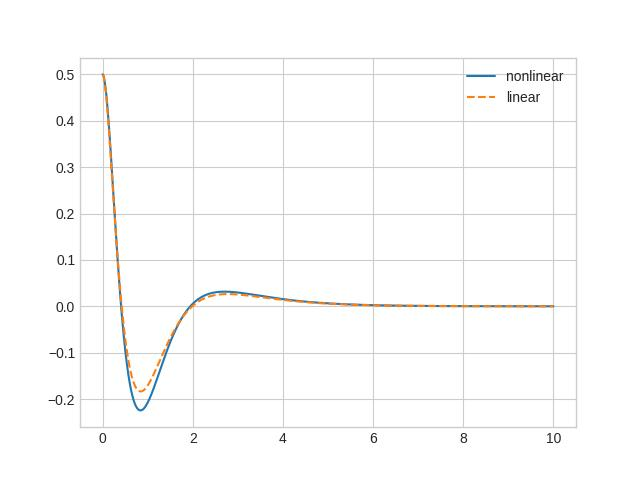
\includegraphics[width=\textwidth]{task6_1_0.1_0.0_0.5_0.0.jpg}
    \caption{Задание 6.1. Динамика контролируемого выхода.}
    \label{fig:task6_1}
\end{figure}
\begin{figure}[]
    \centering
    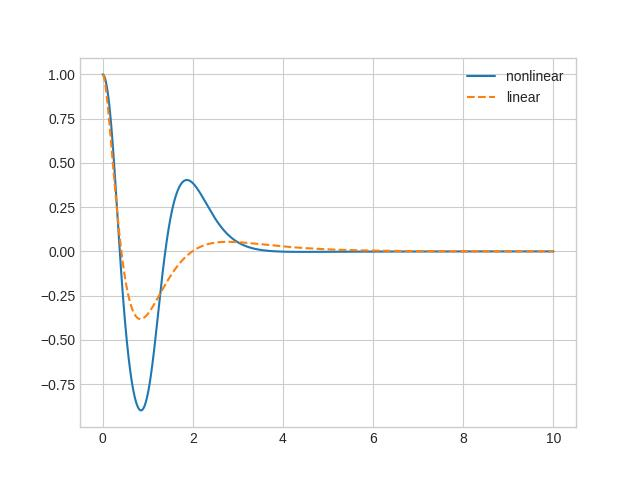
\includegraphics[width=\textwidth]{task6_1_0.1_0.0_1.0_0.0.jpg}
    \caption{Задание 6.1. Динамика контролируемого выхода.}
    \label{fig:task6_1}
\end{figure}

\subsection{Слежение}
Рассмотрим систему:
\begin{equation}
    \begin{cases}
        \dot{x} = A_1x + B_1u \\
        z = C_2x + D_2w
    \end{cases}
\end{equation}
\begin{equation*}
    C_2 = \begin{bmatrix}
        0 & 1 & 0 & 0
    \end{bmatrix},
    D_2 = \begin{bmatrix}
        0.1 & 0.1 & 0.1 & 0.1
    \end{bmatrix}
\end{equation*}
Найдем матрицы регулятора аналогичным способом.
Проведем моделирование:

\begin{figure}[]
    \centering
    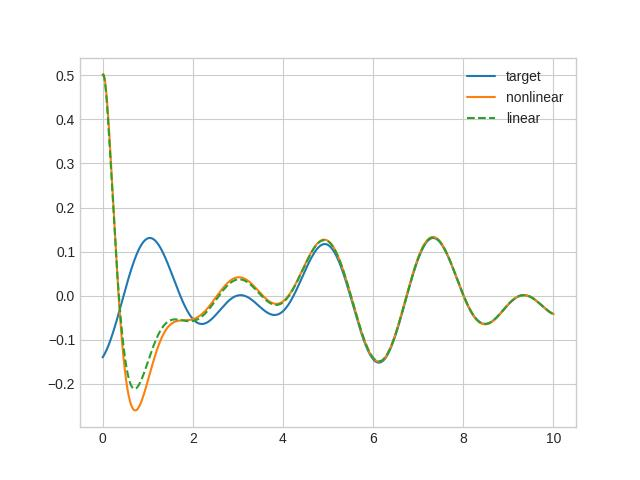
\includegraphics[width=\textwidth]{task6_2_0.0_0.0_0.5_0.3.jpg}
    \caption{Задание 6.2. Динамика контролируемого выхода.}
    \label{fig:task6_1}
\end{figure}
\begin{figure}[]
    \centering
    \includegraphics[width=\textwidth]{task6_2_0.1_0.0_0.1_0.0.jpg}
    \caption{Задание 6.2. Динамика контролируемого выхода.}
    \label{fig:task6_1}
\end{figure}
\begin{figure}[]
    \centering
    \includegraphics[width=\textwidth]{task6_2_0.1_0.0_1.0_0.0.jpg}
    \caption{Задание 6.2. Динамика контролируемого выхода.}
    \label{fig:task6_1}
\end{figure}
Удалось добиться сходимости угла отклонения к заданному закону.

\pagebreak
\section{Итог}
В ходе выполнения проекты были опробованный различные методы управления системами. Каждый имеет свои преимущества и сферы применения. Наиболее универсальным является подход синтеза LQG, т.к. позволяет учесть как внешние возмущения, так и шум датчиков, считая характер помех случайным (что наиболее близко к реальным задачам робототехники).